\documentclass[12pt,a4paper,oneside,english]{article}

\usepackage{tikz}
	\usetikzlibrary{decorations.pathreplacing,intersections,calc,backgrounds,fit}
\usepackage{subcaption}
	\tikzstyle{box}=[rectangle,fill=black!25,minimum size=0.3cm,inner sep=0pt, thick, draw=black, anchor = center]

	\tikzstyle{annot} = [align=center]

\newcommand{\drawtables}[0]
{
  \node[box, minimum width=4.4cm, minimum height=1.6cm, fill=white](table1) at (1,1){};
  \path let \p1 = (table1.south east) in node[box, minimum width=1.6cm, minimum height=2.8cm, fill=white](table2) at (\x1-0.82cm,\y1-1.38cm){};
  \node[annot,below of=table1, xshift=-1.5cm, node distance=1.05cm] {\footnotesize table1};
  \node[annot,below of=table2,  node distance=1.7cm] {\footnotesize table2};
}

\begin{document}
\title{\vspace{-2.2cm}Overview of environments}
%\author{B.Sc.\ Hoai My Van  \\
%	Technische Universit\"at M\"unchen \\
%	}

\date{\vspace{-1.5cm}\today}
\maketitle

\section{Minimal Set-up}
\begin{figure}[!h]
\begin{subfigure}{0.3\textwidth}
\centering
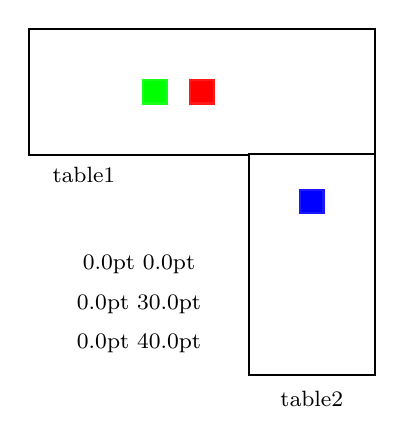
\begin{tikzpicture}
	\coordinate (r) at (0cm, 0cm);
	\coordinate (g) at (0cm, 0.3cm);
	\coordinate (b) at (0cm, 0.4cm);

	\drawtables{}

	\path let \p1 = (table1.center), \p2=(r) in node[box, fill=red, draw=red!90](red) at (\x1-2*\y2,\y1+2*\x2){};
	%\path let \p1 = (table2.center), \p2=(r) in node[box, fill=red, draw=red!90](red) at (\x1+2*\x2,\y1+2*\y2){};
	\path let \p1 = (table1.center), \p2=(g) in node[box, fill=green, draw=green!90](green) at (\x1-2*\y2,\y1+2*\x2){};
	%\path let \p1 = (table2.center), \p2=(g) in node[box, fill=green, draw=green!90](green) at (\x1+2*\x2,\y1+2*\y2){};
	%\path let \p1 = (table1.center), \p2=(b) in node[box, fill=blue, draw=blue!90](blue) at (\x1-2*\y2,\y1+2*\x2){};
	\path let \p1 = (table2.center), \p2=(b) in node[box, fill=blue, draw=blue!90](blue) at (\x1+2*\x2,\y1+2*\y2){};
	
	\path let \p1=(r), \p2=({round(\x1*3.52778)}, {round(\y1*3.52778)}) in node[annot] at(0.2, -1.2){\footnotesize\x2 \y2};
	\path let \p1=(g), \p2=({round(\x1*3.52778)}, {round(\y1*3.52778)}) in node[annot] at(0.2, -1.7){\footnotesize\x2 \y2};
	\path let \p1=(b), \p2=({round(\x1*3.52778)}, {round(\y1*3.52778)}) in node[annot] at(0.2, -2.2){\footnotesize\x2 \y2};

\end{tikzpicture}
\subcaption{Env 001}
\end{subfigure}\hfill
\begin{subfigure}{0.3\textwidth}
\centering
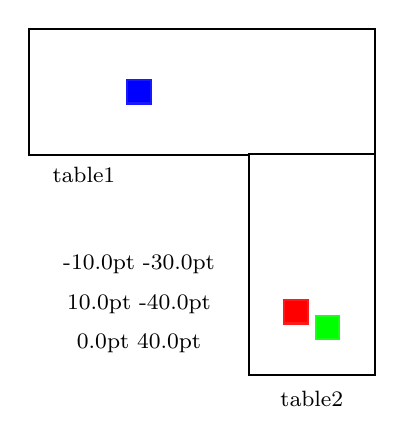
\begin{tikzpicture}
	\coordinate (r) at (-0.1cm, -0.3cm);
	\coordinate (g) at (0.1cm, -0.4cm);
	\coordinate (b) at (0cm, 0.4cm);

	\drawtables{}

	%\path let \p1 = (table1.center), \p2=(r) in node[box, fill=red, draw=red!90](red) at (\x1-2*\y2,\y1+2*\x2){};
	\path let \p1 = (table2.center), \p2=(r) in node[box, fill=red, draw=red!90](red) at (\x1+2*\x2,\y1+2*\y2){};
	%\path let \p1 = (table1.center), \p2=(g) in node[box, fill=green, draw=green!90](green) at (\x1-2*\y2,\y1+2*\x2){};
	\path let \p1 = (table2.center), \p2=(g) in node[box, fill=green, draw=green!90](green) at (\x1+2*\x2,\y1+2*\y2){};
	\path let \p1 = (table1.center), \p2=(b) in node[box, fill=blue, draw=blue!90](blue) at (\x1-2*\y2,\y1+2*\x2){};
	%\path let \p1 = (table2.center), \p2=(b) in node[box, fill=blue, draw=blue!90](blue) at (\x1+2*\x2,\y1+2*\y2){};
	
	\path let \p1=(r), \p2=({round(\x1*3.52778)}, {round(\y1*3.52778)}) in node[annot] at(0.2, -1.2){\footnotesize\x2 \y2};
	\path let \p1=(g), \p2=({round(\x1*3.52778)}, {round(\y1*3.52778)}) in node[annot] at(0.2, -1.7){\footnotesize\x2 \y2};
	\path let \p1=(b), \p2=({round(\x1*3.52778)}, {round(\y1*3.52778)}) in node[annot] at(0.2, -2.2){\footnotesize\x2 \y2};

\end{tikzpicture}
\subcaption{Env 002}
\end{subfigure}\hfill
\begin{subfigure}{0.3\textwidth}
\centering
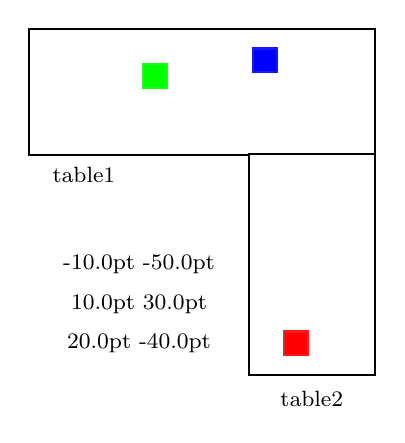
\begin{tikzpicture}
	\coordinate (r) at (-0.1cm, -0.5cm);
	\coordinate (g) at (0.1cm, 0.3cm);
	\coordinate (b) at (0.2cm, -0.4cm);

	\drawtables{}

	%\path let \p1 = (table1.center), \p2=(r) in node[box, fill=red, draw=red!90](red) at (\x1-2*\y2,\y1+2*\x2){};
	\path let \p1 = (table2.center), \p2=(r) in node[box, fill=red, draw=red!90](red) at (\x1+2*\x2,\y1+2*\y2){};
	\path let \p1 = (table1.center), \p2=(g) in node[box, fill=green, draw=green!90](green) at (\x1-2*\y2,\y1+2*\x2){};
	%\path let \p1 = (table2.center), \p2=(g) in node[box, fill=green, draw=green!90](green) at (\x1+2*\x2,\y1+2*\y2){};
	\path let \p1 = (table1.center), \p2=(b) in node[box, fill=blue, draw=blue!90](blue) at (\x1-2*\y2,\y1+2*\x2){};
	%\path let \p1 = (table2.center), \p2=(b) in node[box, fill=blue, draw=blue!90](blue) at (\x1+2*\x2,\y1+2*\y2){};
	
	\path let \p1=(r), \p2=({round(\x1*3.52778)}, {round(\y1*3.52778)}) in node[annot] at(0.2, -1.2){\footnotesize\x2 \y2};
	\path let \p1=(g), \p2=({round(\x1*3.52778)}, {round(\y1*3.52778)}) in node[annot] at(0.2, -1.7){\footnotesize\x2 \y2};
	\path let \p1=(b), \p2=({round(\x1*3.52778)}, {round(\y1*3.52778)}) in node[annot] at(0.2, -2.2){\footnotesize\x2 \y2};

	
\end{tikzpicture}
\subcaption{Env 003}
\end{subfigure}\\

\begin{subfigure}{0.3\textwidth}
\centering
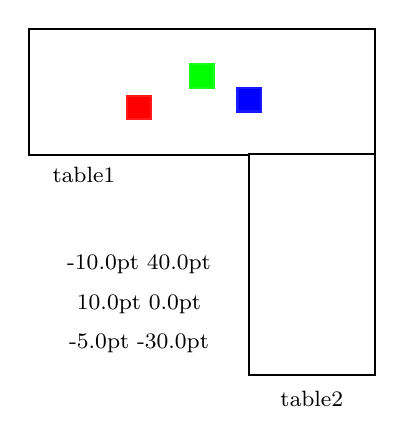
\begin{tikzpicture}
	\coordinate (r) at (-0.1cm, 0.4cm);
	\coordinate (g) at (0.1cm, 0cm);
	\coordinate (b) at (-.05cm, -0.3cm);

	\drawtables{}

	\path let \p1 = (table1.center), \p2=(r) in node[box, fill=red, draw=red!90](red) at (\x1-2*\y2,\y1+2*\x2){};
	%\path let \p1 = (table2.center), \p2=(r) in node[box, fill=red, draw=red!90](red) at (\x1+2*\x2,\y1+2*\y2){};
	\path let \p1 = (table1.center), \p2=(g) in node[box, fill=green, draw=green!90](green) at (\x1-2*\y2,\y1+2*\x2){};
	%\path let \p1 = (table2.center), \p2=(g) in node[box, fill=green, draw=green!90](green) at (\x1+2*\x2,\y1+2*\y2){};
	\path let \p1 = (table1.center), \p2=(b) in node[box, fill=blue, draw=blue!90](blue) at (\x1-2*\y2,\y1+2*\x2){};
	%\path let \p1 = (table2.center), \p2=(b) in node[box, fill=blue, draw=blue!90](blue) at (\x1+2*\x2,\y1+2*\y2){};
	
	\path let \p1=(r), \p2=({round(\x1*3.52778)}, {round(\y1*3.52778)}) in node[annot] at(0.2, -1.2){\footnotesize\x2 \y2};
	\path let \p1=(g), \p2=({round(\x1*3.52778)}, {round(\y1*3.52778)}) in node[annot] at(0.2, -1.7){\footnotesize\x2 \y2};
	\path let \p1=(b), \p2=({round(\x1*3.52778)}, {round(\y1*3.52778)}) in node[annot] at(0.2, -2.2){\footnotesize\x2 \y2};


\end{tikzpicture}
\subcaption{Env 004}
\end{subfigure}\hfill
\begin{subfigure}{0.3\textwidth}
\centering
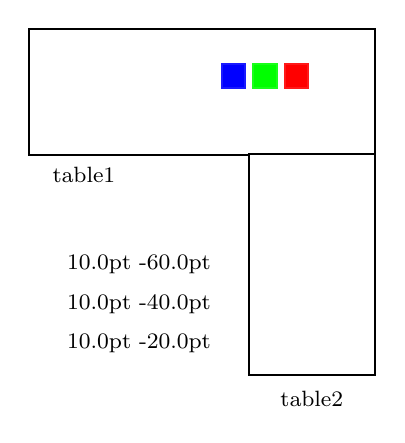
\begin{tikzpicture}
	\coordinate (r) at (0.1cm, -0.6cm);
	\coordinate (g) at (0.1cm, -0.4cm);
	\coordinate (b) at (0.1cm, -0.2cm);

	\drawtables{}

	\path let \p1 = (table1.center), \p2=(r) in node[box, fill=red, draw=red!90](red) at (\x1-2*\y2,\y1+2*\x2){};
	%\path let \p1 = (table2.center), \p2=(r) in node[box, fill=red, draw=red!90](red) at (\x1+2*\x2,\y1+2*\y2){};
	\path let \p1 = (table1.center), \p2=(g) in node[box, fill=green, draw=green!90](green) at (\x1-2*\y2,\y1+2*\x2){};
	%\path let \p1 = (table2.center), \p2=(g) in node[box, fill=green, draw=green!90](green) at (\x1+2*\x2,\y1+2*\y2){};
	\path let \p1 = (table1.center), \p2=(b) in node[box, fill=blue, draw=blue!90](blue) at (\x1-2*\y2,\y1+2*\x2){};
	%\path let \p1 = (table2.center), \p2=(b) in node[box, fill=blue, draw=blue!90](blue) at (\x1+2*\x2,\y1+2*\y2){};
	
	\path let \p1=(r), \p2=({round(\x1*3.52778)}, {round(\y1*3.52778)}) in node[annot] at(0.2, -1.2){\footnotesize\x2 \y2};
	\path let \p1=(g), \p2=({round(\x1*3.52778)}, {round(\y1*3.52778)}) in node[annot] at(0.2, -1.7){\footnotesize\x2 \y2};
	\path let \p1=(b), \p2=({round(\x1*3.52778)}, {round(\y1*3.52778)}) in node[annot] at(0.2, -2.2){\footnotesize\x2 \y2};

\end{tikzpicture}
\subcaption{Env 005}
\end{subfigure}\hfill
\begin{subfigure}{0.3\textwidth}
\centering
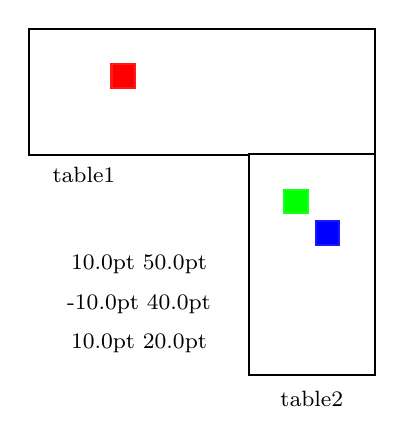
\begin{tikzpicture}
	\coordinate (r) at (0.1cm, 0.5cm);
	\coordinate (g) at (-0.1cm, 0.4cm);
	\coordinate (b) at (0.1cm, 0.2cm);

	\drawtables{}

	\path let \p1 = (table1.center), \p2=(r) in node[box, fill=red, draw=red!90](red) at (\x1-2*\y2,\y1+2*\x2){};
	%\path let \p1 = (table2.center), \p2=(r) in node[box, fill=red, draw=red!90](red) at (\x1+2*\x2,\y1+2*\y2){};
	%\path let \p1 = (table1.center), \p2=(g) in node[box, fill=green, draw=green!90](green) at (\x1-2*\y2,\y1+2*\x2){};
	\path let \p1 = (table2.center), \p2=(g) in node[box, fill=green, draw=green!90](green) at (\x1+2*\x2,\y1+2*\y2){};
	%\path let \p1 = (table1.center), \p2=(b) in node[box, fill=blue, draw=blue!90](blue) at (\x1-2*\y2,\y1+2*\x2){};
	\path let \p1 = (table2.center), \p2=(b) in node[box, fill=blue, draw=blue!90](blue) at (\x1+2*\x2,\y1+2*\y2){};
	
	\path let \p1=(r), \p2=({round(\x1*3.52778)}, {round(\y1*3.52778)}) in node[annot] at(0.2, -1.2){\footnotesize\x2 \y2};
	\path let \p1=(g), \p2=({round(\x1*3.52778)}, {round(\y1*3.52778)}) in node[annot] at(0.2, -1.7){\footnotesize\x2 \y2};
	\path let \p1=(b), \p2=({round(\x1*3.52778)}, {round(\y1*3.52778)}) in node[annot] at(0.2, -2.2){\footnotesize\x2 \y2};

	
\end{tikzpicture}
\subcaption{Env 006}
\end{subfigure}\\


\begin{subfigure}{0.3\textwidth}
\centering
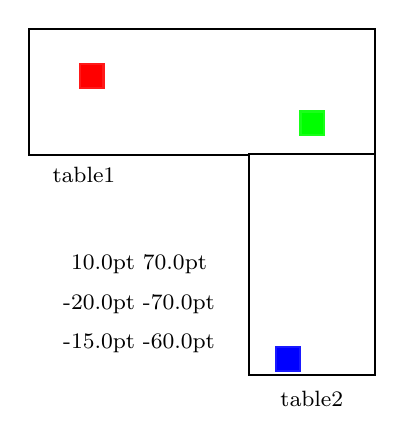
\begin{tikzpicture}
	\coordinate (r) at (0.1cm, 0.7cm);
	\coordinate (g) at (-0.2cm, -0.7cm);
	\coordinate (b) at (-.15cm, -0.6cm);

	\drawtables{}

	\path let \p1 = (table1.center), \p2=(r) in node[box, fill=red, draw=red!90](red) at (\x1-2*\y2,\y1+2*\x2){};
	%\path let \p1 = (table2.center), \p2=(r) in node[box, fill=red, draw=red!90](red) at (\x1+2*\x2,\y1+2*\y2){};
	\path let \p1 = (table1.center), \p2=(g) in node[box, fill=green, draw=green!90](green) at (\x1-2*\y2,\y1+2*\x2){};
	%\path let \p1 = (table2.center), \p2=(g) in node[box, fill=green, draw=green!90](green) at (\x1+2*\x2,\y1+2*\y2){};
	%\path let \p1 = (table1.center), \p2=(b) in node[box, fill=blue, draw=blue!90](blue) at (\x1-2*\y2,\y1+2*\x2){};
	\path let \p1 = (table2.center), \p2=(b) in node[box, fill=blue, draw=blue!90](blue) at (\x1+2*\x2,\y1+2*\y2){};
	
	\path let \p1=(r), \p2=({round(\x1*3.52778)}, {round(\y1*3.52778)}) in node[annot] at(0.2, -1.2){\footnotesize\x2 \y2};
	\path let \p1=(g), \p2=({round(\x1*3.52778)}, {round(\y1*3.52778)}) in node[annot] at(0.2, -1.7){\footnotesize\x2 \y2};
	\path let \p1=(b), \p2=({round(\x1*3.52778)}, {round(\y1*3.52778)}) in node[annot] at(0.2, -2.2){\footnotesize\x2 \y2};


\end{tikzpicture}
\subcaption{Env 007}
\end{subfigure}\hfill
\begin{subfigure}{0.3\textwidth}
\centering
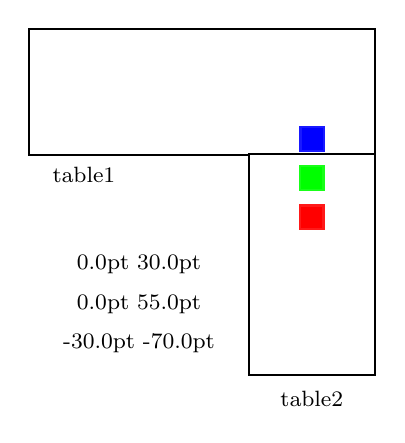
\begin{tikzpicture}
	\coordinate (r) at (0.cm, 0.3cm);
	\coordinate (g) at (0.cm, 0.55cm);
	\coordinate (b) at (-0.3cm, -0.7cm);

	\drawtables{}

	%\path let \p1 = (table1.center), \p2=(r) in node[box, fill=red, draw=red!90](red) at (\x1-2*\y2,\y1+2*\x2){};
	\path let \p1 = (table2.center), \p2=(r) in node[box, fill=red, draw=red!90](red) at (\x1+2*\x2,\y1+2*\y2){};
	%\path let \p1 = (table1.center), \p2=(g) in node[box, fill=green, draw=green!90](green) at (\x1-2*\y2,\y1+2*\x2){};
	\path let \p1 = (table2.center), \p2=(g) in node[box, fill=green, draw=green!90](green) at (\x1+2*\x2,\y1+2*\y2){};
	\path let \p1 = (table1.center), \p2=(b) in node[box, fill=blue, draw=blue!90](blue) at (\x1-2*\y2,\y1+2*\x2){};
	%\path let \p1 = (table2.center), \p2=(b) in node[box, fill=blue, draw=blue!90](blue) at (\x1+2*\x2,\y1+2*\y2){};
	
	\path let \p1=(r), \p2=({round(\x1*3.52778)}, {round(\y1*3.52778)}) in node[annot] at(0.2, -1.2){\footnotesize\x2 \y2};
	\path let \p1=(g), \p2=({round(\x1*3.52778)}, {round(\y1*3.52778)}) in node[annot] at(0.2, -1.7){\footnotesize\x2 \y2};
	\path let \p1=(b), \p2=({round(\x1*3.52778)}, {round(\y1*3.52778)}) in node[annot] at(0.2, -2.2){\footnotesize\x2 \y2};

\end{tikzpicture}
\subcaption{Env 008}
\end{subfigure}\hfill
\begin{subfigure}{0.3\textwidth}
\centering
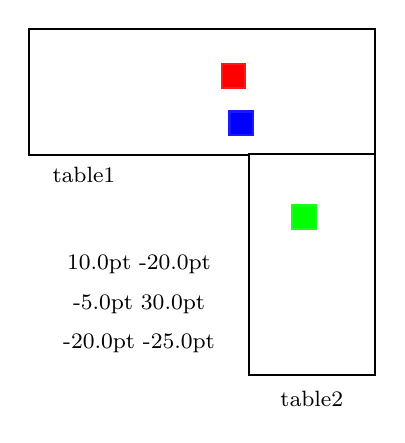
\begin{tikzpicture}
	\coordinate (r) at (0.1cm, -0.2cm);
	\coordinate (g) at (-0.05cm, 0.3cm);
	\coordinate (b) at (-0.2cm, -0.25cm);

	\drawtables{}

	\path let \p1 = (table1.center), \p2=(r) in node[box, fill=red, draw=red!90](red) at (\x1-2*\y2,\y1+2*\x2){};
	%\path let \p1 = (table2.center), \p2=(r) in node[box, fill=red, draw=red!90](red) at (\x1+2*\x2,\y1+2*\y2){};
	%\path let \p1 = (table1.center), \p2=(g) in node[box, fill=green, draw=green!90](green) at (\x1-2*\y2,\y1+2*\x2){};
	\path let \p1 = (table2.center), \p2=(g) in node[box, fill=green, draw=green!90](green) at (\x1+2*\x2,\y1+2*\y2){};
	\path let \p1 = (table1.center), \p2=(b) in node[box, fill=blue, draw=blue!90](blue) at (\x1-2*\y2,\y1+2*\x2){};
	%\path let \p1 = (table2.center), \p2=(b) in node[box, fill=blue, draw=blue!90](blue) at (\x1+2*\x2,\y1+2*\y2){};
	
	\path let \p1=(r), \p2=({round(\x1*3.52778)}, {round(\y1*3.52778)}) in node[annot] at(0.2, -1.2){\footnotesize\x2 \y2};
	\path let \p1=(g), \p2=({round(\x1*3.52778)}, {round(\y1*3.52778)}) in node[annot] at(0.2, -1.7){\footnotesize\x2 \y2};
	\path let \p1=(b), \p2=({round(\x1*3.52778)}, {round(\y1*3.52778)}) in node[annot] at(0.2, -2.2){\footnotesize\x2 \y2};

	
\end{tikzpicture}
\subcaption{Env 009}
\end{subfigure}\\
\end{figure}

\begin{figure}[!h]
\begin{subfigure}{0.3\textwidth}
\centering
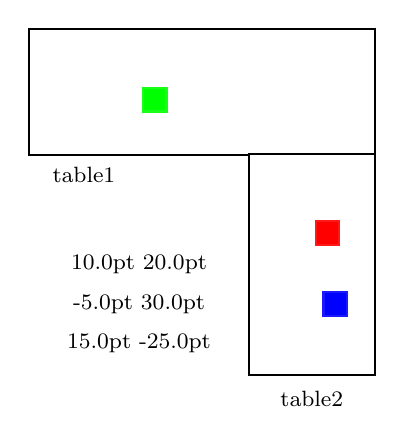
\begin{tikzpicture}
	\coordinate (r) at (0.1cm, 0.2cm);
	\coordinate (g) at (-0.05cm, 0.3cm);
	\coordinate (b) at (0.15cm, -0.25cm);

	\drawtables{}

	%\path let \p1 = (table1.center), \p2=(r) in node[box, fill=red, draw=red!90](red) at (\x1-2*\y2,\y1+2*\x2){};
	\path let \p1 = (table2.center), \p2=(r) in node[box, fill=red, draw=red!90](red) at (\x1+2*\x2,\y1+2*\y2){};
	\path let \p1 = (table1.center), \p2=(g) in node[box, fill=green, draw=green!90](green) at (\x1-2*\y2,\y1+2*\x2){};
	%\path let \p1 = (table2.center), \p2=(g) in node[box, fill=green, draw=green!90](green) at (\x1+2*\x2,\y1+2*\y2){};
	%\path let \p1 = (table1.center), \p2=(b) in node[box, fill=blue, draw=blue!90](blue) at (\x1-2*\y2,\y1+2*\x2){};
	\path let \p1 = (table2.center), \p2=(b) in node[box, fill=blue, draw=blue!90](blue) at (\x1+2*\x2,\y1+2*\y2){};
	
	\path let \p1=(r), \p2=({round(\x1*3.52778)}, {round(\y1*3.52778)}) in node[annot] at(0.2, -1.2){\footnotesize\x2 \y2};
	\path let \p1=(g), \p2=({round(\x1*3.52778)}, {round(\y1*3.52778)}) in node[annot] at(0.2, -1.7){\footnotesize\x2 \y2};
	\path let \p1=(b), \p2=({round(\x1*3.52778)}, {round(\y1*3.52778)}) in node[annot] at(0.2, -2.2){\footnotesize\x2 \y2};


\end{tikzpicture}
\subcaption{Env 010}
\end{subfigure}\hfill
\begin{subfigure}{0.3\textwidth}
\centering
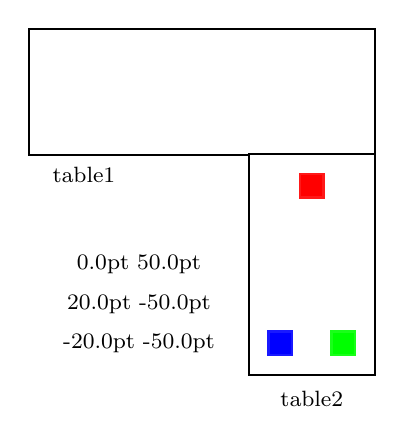
\begin{tikzpicture}
	\coordinate (r) at (0.cm, 0.5cm);
	\coordinate (g) at (0.2cm, -0.5cm);
	\coordinate (b) at (-0.2cm, -0.5cm);

	\drawtables{}

	%\path let \p1 = (table1.center), \p2=(r) in node[box, fill=red, draw=red!90](red) at (\x1-2*\y2,\y1+2*\x2){};
	\path let \p1 = (table2.center), \p2=(r) in node[box, fill=red, draw=red!90](red) at (\x1+2*\x2,\y1+2*\y2){};
	%\path let \p1 = (table1.center), \p2=(g) in node[box, fill=green, draw=green!90](green) at (\x1-2*\y2,\y1+2*\x2){};
	\path let \p1 = (table2.center), \p2=(g) in node[box, fill=green, draw=green!90](green) at (\x1+2*\x2,\y1+2*\y2){};
	%\path let \p1 = (table1.center), \p2=(b) in node[box, fill=blue, draw=blue!90](blue) at (\x1-2*\y2,\y1+2*\x2){};
	\path let \p1 = (table2.center), \p2=(b) in node[box, fill=blue, draw=blue!90](blue) at (\x1+2*\x2,\y1+2*\y2){};
	
	\path let \p1=(r), \p2=({round(\x1*3.52778)}, {round(\y1*3.52778)}) in node[annot] at(0.2, -1.2){\footnotesize\x2 \y2};
	\path let \p1=(g), \p2=({round(\x1*3.52778)}, {round(\y1*3.52778)}) in node[annot] at(0.2, -1.7){\footnotesize\x2 \y2};
	\path let \p1=(b), \p2=({round(\x1*3.52778)}, {round(\y1*3.52778)}) in node[annot] at(0.2, -2.2){\footnotesize\x2 \y2};

\end{tikzpicture}
\subcaption{Env 011}
\end{subfigure}\hfill
\begin{subfigure}{0.3\textwidth}
\centering
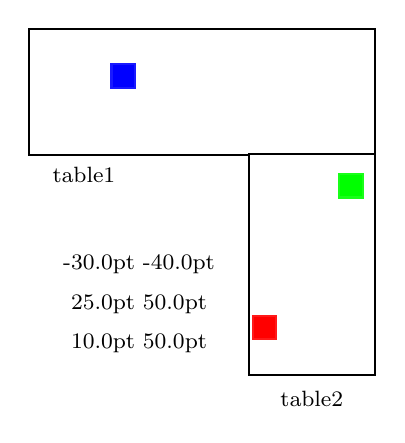
\begin{tikzpicture}
	\coordinate (r) at (-0.3cm, -0.4cm);
	\coordinate (g) at (0.25cm, 0.5cm);
	\coordinate (b) at (0.1cm, 0.5cm);

	\drawtables{}

	%\path let \p1 = (table1.center), \p2=(r) in node[box, fill=red, draw=red!90](red) at (\x1-2*\y2,\y1+2*\x2){};
	\path let \p1 = (table2.center), \p2=(r) in node[box, fill=red, draw=red!90](red) at (\x1+2*\x2,\y1+2*\y2){};
	%\path let \p1 = (table1.center), \p2=(g) in node[box, fill=green, draw=green!90](green) at (\x1-2*\y2,\y1+2*\x2){};
	\path let \p1 = (table2.center), \p2=(g) in node[box, fill=green, draw=green!90](green) at (\x1+2*\x2,\y1+2*\y2){};
	\path let \p1 = (table1.center), \p2=(b) in node[box, fill=blue, draw=blue!90](blue) at (\x1-2*\y2,\y1+2*\x2){};
	%\path let \p1 = (table2.center), \p2=(b) in node[box, fill=blue, draw=blue!90](blue) at (\x1+2*\x2,\y1+2*\y2){};
	
	\path let \p1=(r), \p2=({round(\x1*3.52778)}, {round(\y1*3.52778)}) in node[annot] at(0.2, -1.2){\footnotesize\x2 \y2};
	\path let \p1=(g), \p2=({round(\x1*3.52778)}, {round(\y1*3.52778)}) in node[annot] at(0.2, -1.7){\footnotesize\x2 \y2};
	\path let \p1=(b), \p2=({round(\x1*3.52778)}, {round(\y1*3.52778)}) in node[annot] at(0.2, -2.2){\footnotesize\x2 \y2};

	
\end{tikzpicture}
\subcaption{Env 012}
\end{subfigure}\\

\begin{subfigure}{0.3\textwidth}
\centering
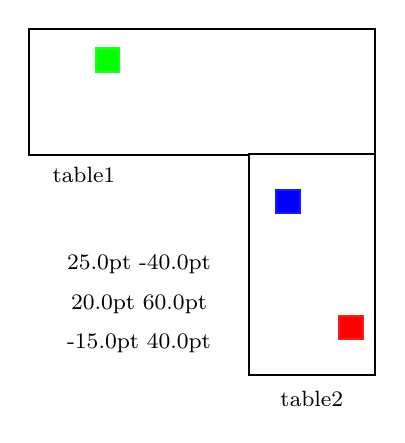
\begin{tikzpicture}
	\coordinate (r) at (0.25cm, -0.4cm);
	\coordinate (g) at (0.2cm, 0.6cm);
	\coordinate (b) at (-.15cm, 0.4cm);

	\drawtables{}

	%\path let \p1 = (table1.center), \p2=(r) in node[box, fill=red, draw=red!90](red) at (\x1-2*\y2,\y1+2*\x2){};
	\path let \p1 = (table2.center), \p2=(r) in node[box, fill=red, draw=red!90](red) at (\x1+2*\x2,\y1+2*\y2){};
	\path let \p1 = (table1.center), \p2=(g) in node[box, fill=green, draw=green!90](green) at (\x1-2*\y2,\y1+2*\x2){};
	%\path let \p1 = (table2.center), \p2=(g) in node[box, fill=green, draw=green!90](green) at (\x1+2*\x2,\y1+2*\y2){};
	%\path let \p1 = (table1.center), \p2=(b) in node[box, fill=blue, draw=blue!90](blue) at (\x1-2*\y2,\y1+2*\x2){};
	\path let \p1 = (table2.center), \p2=(b) in node[box, fill=blue, draw=blue!90](blue) at (\x1+2*\x2,\y1+2*\y2){};
	
	\path let \p1=(r), \p2=({round(\x1*3.52778)}, {round(\y1*3.52778)}) in node[annot] at(0.2, -1.2){\footnotesize\x2 \y2};
	\path let \p1=(g), \p2=({round(\x1*3.52778)}, {round(\y1*3.52778)}) in node[annot] at(0.2, -1.7){\footnotesize\x2 \y2};
	\path let \p1=(b), \p2=({round(\x1*3.52778)}, {round(\y1*3.52778)}) in node[annot] at(0.2, -2.2){\footnotesize\x2 \y2};


\end{tikzpicture}
\subcaption{Env 013}
\end{subfigure}\hfill
\begin{subfigure}{0.3\textwidth}
\centering
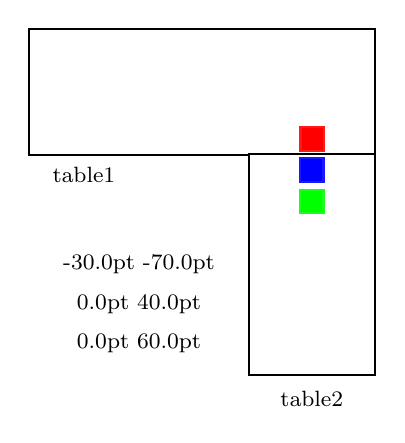
\begin{tikzpicture}
	\coordinate (r) at (-0.3cm, -0.7cm);
	\coordinate (g) at (0cm, 0.4cm);
	\coordinate (b) at (0cm, 0.6cm);

	\drawtables{}

	\path let \p1 = (table1.center), \p2=(r) in node[box, fill=red, draw=red!90](red) at (\x1-2*\y2,\y1+2*\x2){};
	%\path let \p1 = (table2.center), \p2=(r) in node[box, fill=red, draw=red!90](red) at (\x1+2*\x2,\y1+2*\y2){};
	%\path let \p1 = (table1.center), \p2=(g) in node[box, fill=green, draw=green!90](green) at (\x1-2*\y2,\y1+2*\x2){};
	\path let \p1 = (table2.center), \p2=(g) in node[box, fill=green, draw=green!90](green) at (\x1+2*\x2,\y1+2*\y2){};
	%\path let \p1 = (table1.center), \p2=(b) in node[box, fill=blue, draw=blue!90](blue) at (\x1-2*\y2,\y1+2*\x2){};
	\path let \p1 = (table2.center), \p2=(b) in node[box, fill=blue, draw=blue!90](blue) at (\x1+2*\x2,\y1+2*\y2){};
	
	\path let \p1=(r), \p2=({round(\x1*3.52778)}, {round(\y1*3.52778)}) in node[annot] at(0.2, -1.2){\footnotesize\x2 \y2};
	\path let \p1=(g), \p2=({round(\x1*3.52778)}, {round(\y1*3.52778)}) in node[annot] at(0.2, -1.7){\footnotesize\x2 \y2};
	\path let \p1=(b), \p2=({round(\x1*3.52778)}, {round(\y1*3.52778)}) in node[annot] at(0.2, -2.2){\footnotesize\x2 \y2};

\end{tikzpicture}
\subcaption{Env 014}
\end{subfigure}\hfill
\begin{subfigure}{0.3\textwidth}
\centering
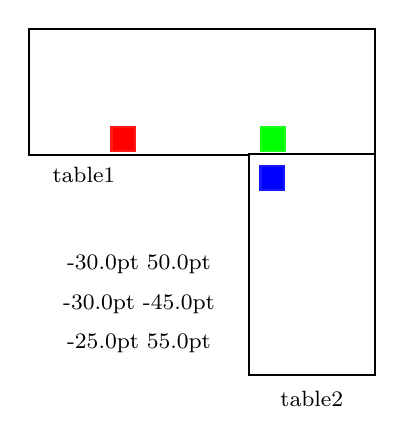
\begin{tikzpicture}
	\coordinate (r) at (-0.3cm, 0.5cm);
	\coordinate (g) at (-0.3cm, -0.45cm);
	\coordinate (b) at (-0.25cm, 0.55cm);

	\drawtables{}

	\path let \p1 = (table1.center), \p2=(r) in node[box, fill=red, draw=red!90](red) at (\x1-2*\y2,\y1+2*\x2){};
	%\path let \p1 = (table2.center), \p2=(r) in node[box, fill=red, draw=red!90](red) at (\x1+2*\x2,\y1+2*\y2){};
	\path let \p1 = (table1.center), \p2=(g) in node[box, fill=green, draw=green!90](green) at (\x1-2*\y2,\y1+2*\x2){};
	%\path let \p1 = (table2.center), \p2=(g) in node[box, fill=green, draw=green!90](green) at (\x1+2*\x2,\y1+2*\y2){};
	%\path let \p1 = (table1.center), \p2=(b) in node[box, fill=blue, draw=blue!90](blue) at (\x1-2*\y2,\y1+2*\x2){};
	\path let \p1 = (table2.center), \p2=(b) in node[box, fill=blue, draw=blue!90](blue) at (\x1+2*\x2,\y1+2*\y2){};
	
	\path let \p1=(r), \p2=({round(\x1*3.52778)}, {round(\y1*3.52778)}) in node[annot] at(0.2, -1.2){\footnotesize\x2 \y2};
	\path let \p1=(g), \p2=({round(\x1*3.52778)}, {round(\y1*3.52778)}) in node[annot] at(0.2, -1.7){\footnotesize\x2 \y2};
	\path let \p1=(b), \p2=({round(\x1*3.52778)}, {round(\y1*3.52778)}) in node[annot] at(0.2, -2.2){\footnotesize\x2 \y2};

	
\end{tikzpicture}
\subcaption{Env 015}
\end{subfigure}\\


\begin{subfigure}{0.3\textwidth}
\centering
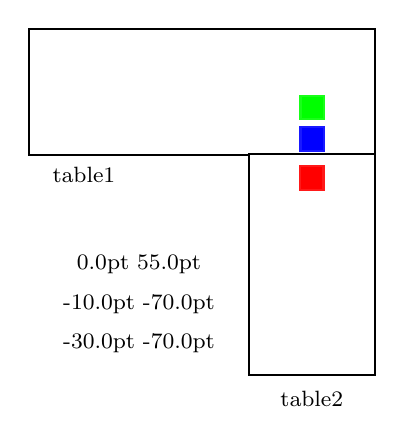
\begin{tikzpicture}
	\coordinate (r) at (0.cm, 0.55cm);
	\coordinate (g) at (-0.1cm, -0.7cm);
	\coordinate (b) at (-.3cm, -0.7cm);

	\drawtables{}

	%\path let \p1 = (table1.center), \p2=(r) in node[box, fill=red, draw=red!90](red) at (\x1-2*\y2,\y1+2*\x2){};
	\path let \p1 = (table2.center), \p2=(r) in node[box, fill=red, draw=red!90](red) at (\x1+2*\x2,\y1+2*\y2){};
	\path let \p1 = (table1.center), \p2=(g) in node[box, fill=green, draw=green!90](green) at (\x1-2*\y2,\y1+2*\x2){};
	%\path let \p1 = (table2.center), \p2=(g) in node[box, fill=green, draw=green!90](green) at (\x1+2*\x2,\y1+2*\y2){};
	\path let \p1 = (table1.center), \p2=(b) in node[box, fill=blue, draw=blue!90](blue) at (\x1-2*\y2,\y1+2*\x2){};
	%\path let \p1 = (table2.center), \p2=(b) in node[box, fill=blue, draw=blue!90](blue) at (\x1+2*\x2,\y1+2*\y2){};
	
	\path let \p1=(r), \p2=({round(\x1*3.52778)}, {round(\y1*3.52778)}) in node[annot] at(0.2, -1.2){\footnotesize\x2 \y2};
	\path let \p1=(g), \p2=({round(\x1*3.52778)}, {round(\y1*3.52778)}) in node[annot] at(0.2, -1.7){\footnotesize\x2 \y2};
	\path let \p1=(b), \p2=({round(\x1*3.52778)}, {round(\y1*3.52778)}) in node[annot] at(0.2, -2.2){\footnotesize\x2 \y2};


\end{tikzpicture}
\subcaption{Env 016}
\end{subfigure}\hfill
\begin{subfigure}{0.3\textwidth}
\centering
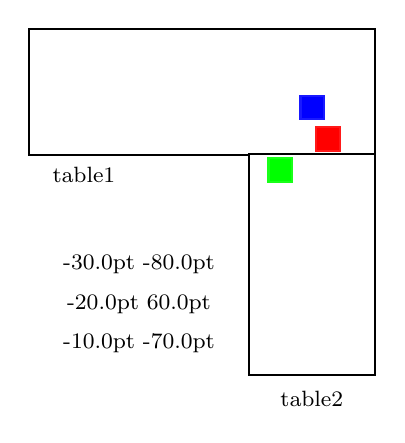
\begin{tikzpicture}
	\coordinate (r) at (-0.3cm, -0.8cm);
	\coordinate (g) at (-0.2cm, 0.6cm);
	\coordinate (b) at (-0.1cm, -0.7cm);

	\drawtables{}

	\path let \p1 = (table1.center), \p2=(r) in node[box, fill=red, draw=red!90](red) at (\x1-2*\y2,\y1+2*\x2){};
	%\path let \p1 = (table2.center), \p2=(r) in node[box, fill=red, draw=red!90](red) at (\x1+2*\x2,\y1+2*\y2){};
	%\path let \p1 = (table1.center), \p2=(g) in node[box, fill=green, draw=green!90](green) at (\x1-2*\y2,\y1+2*\x2){};
	\path let \p1 = (table2.center), \p2=(g) in node[box, fill=green, draw=green!90](green) at (\x1+2*\x2,\y1+2*\y2){};
	\path let \p1 = (table1.center), \p2=(b) in node[box, fill=blue, draw=blue!90](blue) at (\x1-2*\y2,\y1+2*\x2){};
	%\path let \p1 = (table2.center), \p2=(b) in node[box, fill=blue, draw=blue!90](blue) at (\x1+2*\x2,\y1+2*\y2){};
	
	\path let \p1=(r), \p2=({round(\x1*3.52778)}, {round(\y1*3.52778)}) in node[annot] at(0.2, -1.2){\footnotesize\x2 \y2};
	\path let \p1=(g), \p2=({round(\x1*3.52778)}, {round(\y1*3.52778)}) in node[annot] at(0.2, -1.7){\footnotesize\x2 \y2};
	\path let \p1=(b), \p2=({round(\x1*3.52778)}, {round(\y1*3.52778)}) in node[annot] at(0.2, -2.2){\footnotesize\x2 \y2};

\end{tikzpicture}
\subcaption{Env 017}
\end{subfigure}\hfill
\begin{subfigure}{0.3\textwidth}
\centering
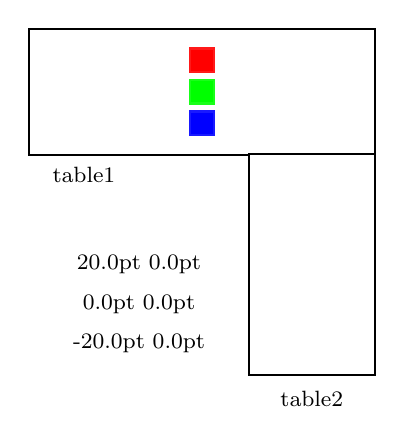
\begin{tikzpicture}
	\coordinate (r) at (0.2cm, 0.cm);
	\coordinate (g) at (0cm, 0cm);
	\coordinate (b) at (-0.2cm, -0cm);

	\drawtables{}

	\path let \p1 = (table1.center), \p2=(r) in node[box, fill=red, draw=red!90](red) at (\x1-2*\y2,\y1+2*\x2){};
	%\path let \p1 = (table2.center), \p2=(r) in node[box, fill=red, draw=red!90](red) at (\x1+2*\x2,\y1+2*\y2){};
	\path let \p1 = (table1.center), \p2=(g) in node[box, fill=green, draw=green!90](green) at (\x1-2*\y2,\y1+2*\x2){};
	%\path let \p1 = (table2.center), \p2=(g) in node[box, fill=green, draw=green!90](green) at (\x1+2*\x2,\y1+2*\y2){};
	\path let \p1 = (table1.center), \p2=(b) in node[box, fill=blue, draw=blue!90](blue) at (\x1-2*\y2,\y1+2*\x2){};
	%\path let \p1 = (table2.center), \p2=(b) in node[box, fill=blue, draw=blue!90](blue) at (\x1+2*\x2,\y1+2*\y2){};
	
	\path let \p1=(r), \p2=({round(\x1*3.52778)}, {round(\y1*3.52778)}) in node[annot] at(0.2, -1.2){\footnotesize\x2 \y2};
	\path let \p1=(g), \p2=({round(\x1*3.52778)}, {round(\y1*3.52778)}) in node[annot] at(0.2, -1.7){\footnotesize\x2 \y2};
	\path let \p1=(b), \p2=({round(\x1*3.52778)}, {round(\y1*3.52778)}) in node[annot] at(0.2, -2.2){\footnotesize\x2 \y2};

	
\end{tikzpicture}
\subcaption{Env 018}
\end{subfigure}\\
\end{figure}

\begin{figure}[!h]
\begin{subfigure}{0.3\textwidth}
\centering
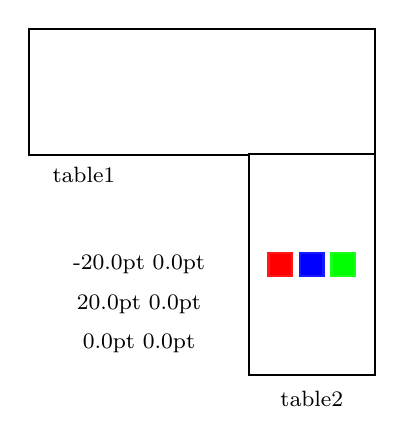
\begin{tikzpicture}
	\coordinate (r) at (-0.2cm, 0cm);
	\coordinate (g) at (0.2cm, 0cm);
	\coordinate (b) at (0cm, 0cm);

	\drawtables{}

	%\path let \p1 = (table1.center), \p2=(r) in node[box, fill=red, draw=red!90](red) at (\x1-2*\y2,\y1+2*\x2){};
	\path let \p1 = (table2.center), \p2=(r) in node[box, fill=red, draw=red!90](red) at (\x1+2*\x2,\y1+2*\y2){};
	%\path let \p1 = (table1.center), \p2=(g) in node[box, fill=green, draw=green!90](green) at (\x1-2*\y2,\y1+2*\x2){};
	\path let \p1 = (table2.center), \p2=(g) in node[box, fill=green, draw=green!90](green) at (\x1+2*\x2,\y1+2*\y2){};
	%\path let \p1 = (table1.center), \p2=(b) in node[box, fill=blue, draw=blue!90](blue) at (\x1-2*\y2,\y1+2*\x2){};
	\path let \p1 = (table2.center), \p2=(b) in node[box, fill=blue, draw=blue!90](blue) at (\x1+2*\x2,\y1+2*\y2){};
	
	\path let \p1=(r), \p2=({round(\x1*3.52778)}, {round(\y1*3.52778)}) in node[annot] at(0.2, -1.2){\footnotesize\x2 \y2};
	\path let \p1=(g), \p2=({round(\x1*3.52778)}, {round(\y1*3.52778)}) in node[annot] at(0.2, -1.7){\footnotesize\x2 \y2};
	\path let \p1=(b), \p2=({round(\x1*3.52778)}, {round(\y1*3.52778)}) in node[annot] at(0.2, -2.2){\footnotesize\x2 \y2};

\end{tikzpicture}
\subcaption{Env 019}
\end{subfigure}\hfill
\begin{subfigure}{0.3\textwidth}
\centering
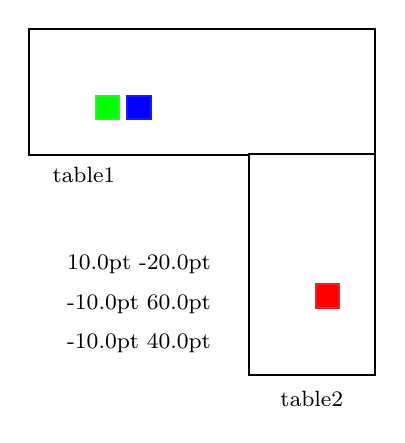
\begin{tikzpicture}
	\coordinate (r) at (0.1cm, -0.2cm);
	\coordinate (g) at (-0.1cm, 0.6cm);
	\coordinate (b) at (-0.1cm, 0.4cm);

	\drawtables{}

	%\path let \p1 = (table1.center), \p2=(r) in node[box, fill=red, draw=red!90](red) at (\x1-2*\y2,\y1+2*\x2){};
	\path let \p1 = (table2.center), \p2=(r) in node[box, fill=red, draw=red!90](red) at (\x1+2*\x2,\y1+2*\y2){};
	\path let \p1 = (table1.center), \p2=(g) in node[box, fill=green, draw=green!90](green) at (\x1-2*\y2,\y1+2*\x2){};
	%\path let \p1 = (table2.center), \p2=(g) in node[box, fill=green, draw=green!90](green) at (\x1+2*\x2,\y1+2*\y2){};
	\path let \p1 = (table1.center), \p2=(b) in node[box, fill=blue, draw=blue!90](blue) at (\x1-2*\y2,\y1+2*\x2){};
	%\path let \p1 = (table2.center), \p2=(b) in node[box, fill=blue, draw=blue!90](blue) at (\x1+2*\x2,\y1+2*\y2){};
	
	\path let \p1=(r), \p2=({round(\x1*3.52778)}, {round(\y1*3.52778)}) in node[annot] at(0.2, -1.2){\footnotesize\x2 \y2};
	\path let \p1=(g), \p2=({round(\x1*3.52778)}, {round(\y1*3.52778)}) in node[annot] at(0.2, -1.7){\footnotesize\x2 \y2};
	\path let \p1=(b), \p2=({round(\x1*3.52778)}, {round(\y1*3.52778)}) in node[annot] at(0.2, -2.2){\footnotesize\x2 \y2};

\end{tikzpicture}
\subcaption{Env 020}
\end{subfigure}\hfill
\begin{subfigure}{0.3\textwidth}
\centering
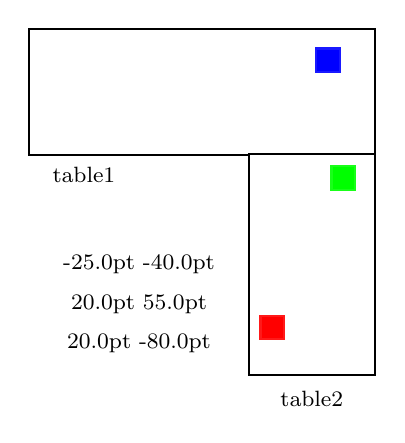
\begin{tikzpicture}
	\coordinate (r) at (-0.25cm, -0.4cm);
	\coordinate (g) at (0.2cm, 0.55cm);
	\coordinate (b) at (0.2cm, -0.8cm);

	\drawtables{}

	%\path let \p1 = (table1.center), \p2=(r) in node[box, fill=red, draw=red!90](red) at (\x1-2*\y2,\y1+2*\x2){};
	\path let \p1 = (table2.center), \p2=(r) in node[box, fill=red, draw=red!90](red) at (\x1+2*\x2,\y1+2*\y2){};
	%\path let \p1 = (table1.center), \p2=(g) in node[box, fill=green, draw=green!90](green) at (\x1-2*\y2,\y1+2*\x2){};
	\path let \p1 = (table2.center), \p2=(g) in node[box, fill=green, draw=green!90](green) at (\x1+2*\x2,\y1+2*\y2){};
	\path let \p1 = (table1.center), \p2=(b) in node[box, fill=blue, draw=blue!90](blue) at (\x1-2*\y2,\y1+2*\x2){};
	%\path let \p1 = (table2.center), \p2=(b) in node[box, fill=blue, draw=blue!90](blue) at (\x1+2*\x2,\y1+2*\y2){};
	
	\path let \p1=(r), \p2=({round(\x1*3.52778)}, {round(\y1*3.52778)}) in node[annot] at(0.2, -1.2){\footnotesize\x2 \y2};
	\path let \p1=(g), \p2=({round(\x1*3.52778)}, {round(\y1*3.52778)}) in node[annot] at(0.2, -1.7){\footnotesize\x2 \y2};
	\path let \p1=(b), \p2=({round(\x1*3.52778)}, {round(\y1*3.52778)}) in node[annot] at(0.2, -2.2){\footnotesize\x2 \y2};

	
\end{tikzpicture}
\subcaption{Env 021}
\end{subfigure}\\

\begin{subfigure}{0.3\textwidth}
\centering
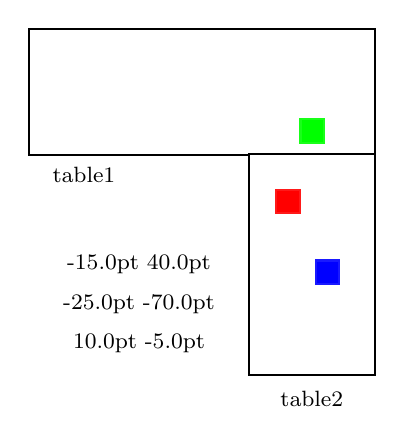
\begin{tikzpicture}
	\coordinate (r) at (-0.15cm, 0.4cm);
	\coordinate (g) at (-0.25cm, -0.7cm);
	\coordinate (b) at (.1cm, -0.05cm);

	\drawtables{}

	%\path let \p1 = (table1.center), \p2=(r) in node[box, fill=red, draw=red!90](red) at (\x1-2*\y2,\y1+2*\x2){};
	\path let \p1 = (table2.center), \p2=(r) in node[box, fill=red, draw=red!90](red) at (\x1+2*\x2,\y1+2*\y2){};
	\path let \p1 = (table1.center), \p2=(g) in node[box, fill=green, draw=green!90](green) at (\x1-2*\y2,\y1+2*\x2){};
	%\path let \p1 = (table2.center), \p2=(g) in node[box, fill=green, draw=green!90](green) at (\x1+2*\x2,\y1+2*\y2){};
	%\path let \p1 = (table1.center), \p2=(b) in node[box, fill=blue, draw=blue!90](blue) at (\x1-2*\y2,\y1+2*\x2){};
	\path let \p1 = (table2.center), \p2=(b) in node[box, fill=blue, draw=blue!90](blue) at (\x1+2*\x2,\y1+2*\y2){};
	
	\path let \p1=(r), \p2=({round(\x1*3.52778)}, {round(\y1*3.52778)}) in node[annot] at(0.2, -1.2){\footnotesize\x2 \y2};
	\path let \p1=(g), \p2=({round(\x1*3.52778)}, {round(\y1*3.52778)}) in node[annot] at(0.2, -1.7){\footnotesize\x2 \y2};
	\path let \p1=(b), \p2=({round(\x1*3.52778)}, {round(\y1*3.52778)}) in node[annot] at(0.2, -2.2){\footnotesize\x2 \y2};


\end{tikzpicture}
\subcaption{Env 022}
\end{subfigure}\hfill
\begin{subfigure}{0.3\textwidth}
\centering
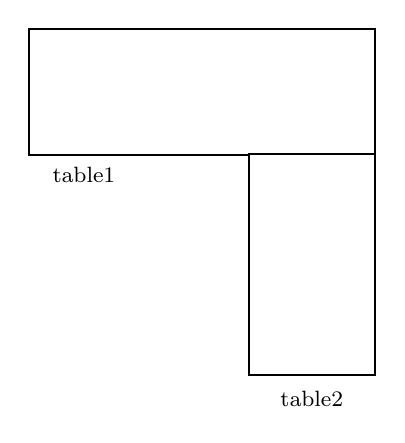
\begin{tikzpicture}
	\coordinate (r) at (0.1cm, -0.6cm);
	\coordinate (g) at (0.1cm, -0.4cm);
	\coordinate (b) at (0.1cm, -0.2cm);

	\drawtables{}

	%\path let \p1 = (table1.center), \p2=(r) in node[box, fill=red, draw=red!90](red) at (\x1-2*\y2,\y1+2*\x2){};
	%\path let \p1 = (table2.center), \p2=(r) in node[box, fill=red, draw=red!90](red) at (\x1+2*\x2,\y1+2*\y2){};
	%\path let \p1 = (table1.center), \p2=(g) in node[box, fill=green, draw=green!90](green) at (\x1-2*\y2,\y1+2*\x2){};
	%\path let \p1 = (table2.center), \p2=(g) in node[box, fill=green, draw=green!90](green) at (\x1+2*\x2,\y1+2*\y2){};
	%\path let \p1 = (table1.center), \p2=(b) in node[box, fill=blue, draw=blue!90](blue) at (\x1-2*\y2,\y1+2*\x2){};
	%\path let \p1 = (table2.center), \p2=(b) in node[box, fill=blue, draw=blue!90](blue) at (\x1+2*\x2,\y1+2*\y2){};
	
	%\path let \p1=(r), \p2=({round(\x1*3.52778)}, {round(\y1*3.52778)}) in node[annot] at(0.2, -1.2){\footnotesize\x2 \y2};
	%\path let \p1=(g), \p2=({round(\x1*3.52778)}, {round(\y1*3.52778)}) in node[annot] at(0.2, -1.7){\footnotesize\x2 \y2};
	%\path let \p1=(b), \p2=({round(\x1*3.52778)}, {round(\y1*3.52778)}) in node[annot] at(0.2, -2.2){\footnotesize\x2 \y2};

\end{tikzpicture}
\subcaption{Env 023}
\end{subfigure}\hfill
\begin{subfigure}{0.3\textwidth}
\centering
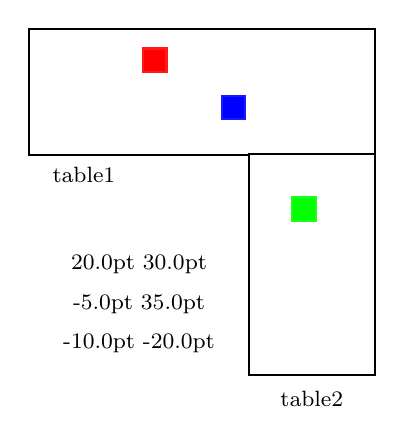
\begin{tikzpicture}
	\coordinate (r) at (0.2cm, 0.3cm);
	\coordinate (g) at (-0.05cm, 0.35cm);
	\coordinate (b) at (-0.1cm, -0.2cm);

	\drawtables{}

	\path let \p1 = (table1.center), \p2=(r) in node[box, fill=red, draw=red!90](red) at (\x1-2*\y2,\y1+2*\x2){};
	%\path let \p1 = (table2.center), \p2=(r) in node[box, fill=red, draw=red!90](red) at (\x1+2*\x2,\y1+2*\y2){};
	%\path let \p1 = (table1.center), \p2=(g) in node[box, fill=green, draw=green!90](green) at (\x1-2*\y2,\y1+2*\x2){};
	\path let \p1 = (table2.center), \p2=(g) in node[box, fill=green, draw=green!90](green) at (\x1+2*\x2,\y1+2*\y2){};
	\path let \p1 = (table1.center), \p2=(b) in node[box, fill=blue, draw=blue!90](blue) at (\x1-2*\y2,\y1+2*\x2){};
	%\path let \p1 = (table2.center), \p2=(b) in node[box, fill=blue, draw=blue!90](blue) at (\x1+2*\x2,\y1+2*\y2){};
	
	\path let \p1=(r), \p2=({round(\x1*3.52778)}, {round(\y1*3.52778)}) in node[annot] at(0.2, -1.2){\footnotesize\x2 \y2};
	\path let \p1=(g), \p2=({round(\x1*3.52778)}, {round(\y1*3.52778)}) in node[annot] at(0.2, -1.7){\footnotesize\x2 \y2};
	\path let \p1=(b), \p2=({round(\x1*3.52778)}, {round(\y1*3.52778)}) in node[annot] at(0.2, -2.2){\footnotesize\x2 \y2};

	
\end{tikzpicture}
\subcaption{Env 024}
\end{subfigure}\\


\begin{subfigure}{0.3\textwidth}
\centering
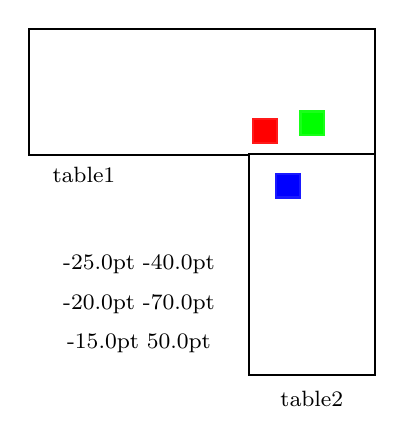
\begin{tikzpicture}
	\coordinate (r) at (-0.25cm, -0.4cm);
	\coordinate (g) at (-0.2cm, -0.7cm);
	\coordinate (b) at (-.15cm, 0.5cm);

	\drawtables{}

	\path let \p1 = (table1.center), \p2=(r) in node[box, fill=red, draw=red!90](red) at (\x1-2*\y2,\y1+2*\x2){};
	%\path let \p1 = (table2.center), \p2=(r) in node[box, fill=red, draw=red!90](red) at (\x1+2*\x2,\y1+2*\y2){};
	\path let \p1 = (table1.center), \p2=(g) in node[box, fill=green, draw=green!90](green) at (\x1-2*\y2,\y1+2*\x2){};
	%\path let \p1 = (table2.center), \p2=(g) in node[box, fill=green, draw=green!90](green) at (\x1+2*\x2,\y1+2*\y2){};
	%\path let \p1 = (table1.center), \p2=(b) in node[box, fill=blue, draw=blue!90](blue) at (\x1-2*\y2,\y1+2*\x2){};
	\path let \p1 = (table2.center), \p2=(b) in node[box, fill=blue, draw=blue!90](blue) at (\x1+2*\x2,\y1+2*\y2){};
	
	\path let \p1=(r), \p2=({round(\x1*3.52778)}, {round(\y1*3.52778)}) in node[annot] at(0.2, -1.2){\footnotesize\x2 \y2};
	\path let \p1=(g), \p2=({round(\x1*3.52778)}, {round(\y1*3.52778)}) in node[annot] at(0.2, -1.7){\footnotesize\x2 \y2};
	\path let \p1=(b), \p2=({round(\x1*3.52778)}, {round(\y1*3.52778)}) in node[annot] at(0.2, -2.2){\footnotesize\x2 \y2};


\end{tikzpicture}
\subcaption{Env 025}
\end{subfigure}\hfill
\begin{subfigure}{0.3\textwidth}
\centering
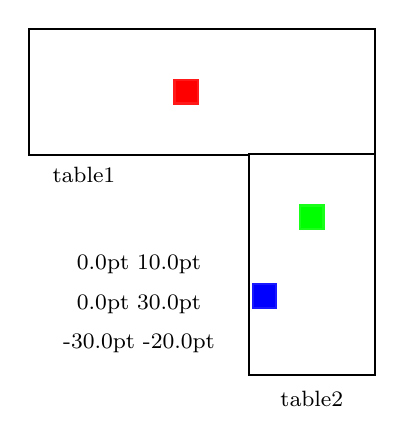
\begin{tikzpicture}
	\coordinate (r) at (0.cm, 0.1cm);
	\coordinate (g) at (0.cm, 0.3cm);
	\coordinate (b) at (-0.3cm, -.2cm);

	\drawtables{}

	\path let \p1 = (table1.center), \p2=(r) in node[box, fill=red, draw=red!90](red) at (\x1-2*\y2,\y1+2*\x2){};
	%\path let \p1 = (table2.center), \p2=(r) in node[box, fill=red, draw=red!90](red) at (\x1+2*\x2,\y1+2*\y2){};
	%\path let \p1 = (table1.center), \p2=(g) in node[box, fill=green, draw=green!90](green) at (\x1-2*\y2,\y1+2*\x2){};
	\path let \p1 = (table2.center), \p2=(g) in node[box, fill=green, draw=green!90](green) at (\x1+2*\x2,\y1+2*\y2){};
	%\path let \p1 = (table1.center), \p2=(b) in node[box, fill=blue, draw=blue!90](blue) at (\x1-2*\y2,\y1+2*\x2){};
	\path let \p1 = (table2.center), \p2=(b) in node[box, fill=blue, draw=blue!90](blue) at (\x1+2*\x2,\y1+2*\y2){};
	
	\path let \p1=(r), \p2=({round(\x1*3.52778)}, {round(\y1*3.52778)}) in node[annot] at(0.2, -1.2){\footnotesize\x2 \y2};
	\path let \p1=(g), \p2=({round(\x1*3.52778)}, {round(\y1*3.52778)}) in node[annot] at(0.2, -1.7){\footnotesize\x2 \y2};
	\path let \p1=(b), \p2=({round(\x1*3.52778)}, {round(\y1*3.52778)}) in node[annot] at(0.2, -2.2){\footnotesize\x2 \y2};

\end{tikzpicture}
\subcaption{Env 026}
\end{subfigure}\hfill
\begin{subfigure}{0.3\textwidth}
\centering
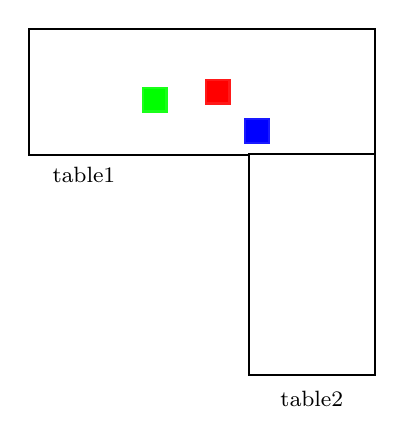
\begin{tikzpicture}
	\coordinate (r) at (0.0cm, -0.1cm);
	\coordinate (g) at (-0.05cm, 0.3cm);
	\coordinate (b) at (-0.25cm, -0.35cm);

	\drawtables{}

	\path let \p1 = (table1.center), \p2=(r) in node[box, fill=red, draw=red!90](red) at (\x1-2*\y2,\y1+2*\x2){};
	%\path let \p1 = (table2.center), \p2=(r) in node[box, fill=red, draw=red!90](red) at (\x1+2*\x2,\y1+2*\y2){};
	\path let \p1 = (table1.center), \p2=(g) in node[box, fill=green, draw=green!90](green) at (\x1-2*\y2,\y1+2*\x2){};
	%\path let \p1 = (table2.center), \p2=(g) in node[box, fill=green, draw=green!90](green) at (\x1+2*\x2,\y1+2*\y2){};
	\path let \p1 = (table1.center), \p2=(b) in node[box, fill=blue, draw=blue!90](blue) at (\x1-2*\y2,\y1+2*\x2){};
	%\path let \p1 = (table2.center), \p2=(b) in node[box, fill=blue, draw=blue!90](blue) at (\x1+2*\x2,\y1+2*\y2){};
	
	%\path let \p1=(r), \p2=({round(\x1*3.52778)}, {round(\y1*3.52778)}) in node[annot] at(0.2, -1.2){\footnotesize\x2 \y2};
	%\path let \p1=(g), \p2=({round(\x1*3.52778)}, {round(\y1*3.52778)}) in node[annot] at(0.2, -1.7){\footnotesize\x2 \y2};
	%\path let \p1=(b), \p2=({round(\x1*3.52778)}, {round(\y1*3.52778)}) in node[annot] at(0.2, -2.2){\footnotesize\x2 \y2};

	
\end{tikzpicture}
\subcaption{Env 027}
\end{subfigure}\\
\end{figure}

\begin{figure}[!h]
\begin{subfigure}{0.3\textwidth}
\centering
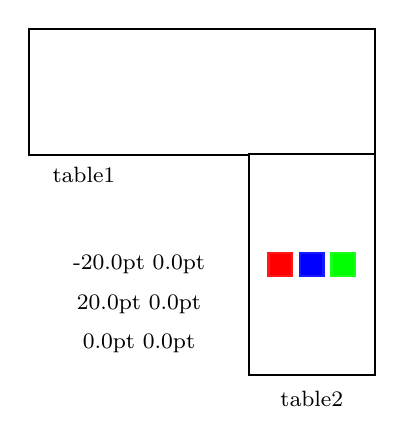
\begin{tikzpicture}
	\coordinate (r) at (-0.2cm, 0cm);
	\coordinate (g) at (0.2cm, 0cm);
	\coordinate (b) at (0cm, 0cm);

	\drawtables{}

	%\path let \p1 = (table1.center), \p2=(r) in node[box, fill=red, draw=red!90](red) at (\x1-2*\y2,\y1+2*\x2){};
	\path let \p1 = (table2.center), \p2=(r) in node[box, fill=red, draw=red!90](red) at (\x1+2*\x2,\y1+2*\y2){};
	%\path let \p1 = (table1.center), \p2=(g) in node[box, fill=green, draw=green!90](green) at (\x1-2*\y2,\y1+2*\x2){};
	\path let \p1 = (table2.center), \p2=(g) in node[box, fill=green, draw=green!90](green) at (\x1+2*\x2,\y1+2*\y2){};
	%\path let \p1 = (table1.center), \p2=(b) in node[box, fill=blue, draw=blue!90](blue) at (\x1-2*\y2,\y1+2*\x2){};
	\path let \p1 = (table2.center), \p2=(b) in node[box, fill=blue, draw=blue!90](blue) at (\x1+2*\x2,\y1+2*\y2){};
	
	\path let \p1=(r), \p2=({round(\x1*3.52778)}, {round(\y1*3.52778)}) in node[annot] at(0.2, -1.2){\footnotesize\x2 \y2};
	\path let \p1=(g), \p2=({round(\x1*3.52778)}, {round(\y1*3.52778)}) in node[annot] at(0.2, -1.7){\footnotesize\x2 \y2};
	\path let \p1=(b), \p2=({round(\x1*3.52778)}, {round(\y1*3.52778)}) in node[annot] at(0.2, -2.2){\footnotesize\x2 \y2};

\end{tikzpicture}
\subcaption{Env 019}
\end{subfigure}\hfill
\begin{subfigure}{0.3\textwidth}
\centering
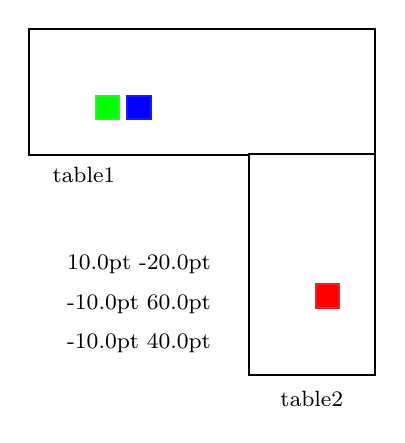
\begin{tikzpicture}
	\coordinate (r) at (0.1cm, -0.2cm);
	\coordinate (g) at (-0.1cm, 0.6cm);
	\coordinate (b) at (-0.1cm, 0.4cm);

	\drawtables{}

	%\path let \p1 = (table1.center), \p2=(r) in node[box, fill=red, draw=red!90](red) at (\x1-2*\y2,\y1+2*\x2){};
	\path let \p1 = (table2.center), \p2=(r) in node[box, fill=red, draw=red!90](red) at (\x1+2*\x2,\y1+2*\y2){};
	\path let \p1 = (table1.center), \p2=(g) in node[box, fill=green, draw=green!90](green) at (\x1-2*\y2,\y1+2*\x2){};
	%\path let \p1 = (table2.center), \p2=(g) in node[box, fill=green, draw=green!90](green) at (\x1+2*\x2,\y1+2*\y2){};
	\path let \p1 = (table1.center), \p2=(b) in node[box, fill=blue, draw=blue!90](blue) at (\x1-2*\y2,\y1+2*\x2){};
	%\path let \p1 = (table2.center), \p2=(b) in node[box, fill=blue, draw=blue!90](blue) at (\x1+2*\x2,\y1+2*\y2){};
	
	\path let \p1=(r), \p2=({round(\x1*3.52778)}, {round(\y1*3.52778)}) in node[annot] at(0.2, -1.2){\footnotesize\x2 \y2};
	\path let \p1=(g), \p2=({round(\x1*3.52778)}, {round(\y1*3.52778)}) in node[annot] at(0.2, -1.7){\footnotesize\x2 \y2};
	\path let \p1=(b), \p2=({round(\x1*3.52778)}, {round(\y1*3.52778)}) in node[annot] at(0.2, -2.2){\footnotesize\x2 \y2};

\end{tikzpicture}
\subcaption{Env 020}
\end{subfigure}\hfill
\begin{subfigure}{0.3\textwidth}
\centering
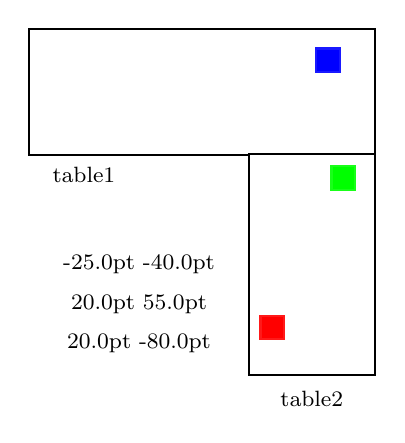
\begin{tikzpicture}
	\coordinate (r) at (-0.25cm, -0.4cm);
	\coordinate (g) at (0.2cm, 0.55cm);
	\coordinate (b) at (0.2cm, -0.8cm);

	\drawtables{}

	%\path let \p1 = (table1.center), \p2=(r) in node[box, fill=red, draw=red!90](red) at (\x1-2*\y2,\y1+2*\x2){};
	\path let \p1 = (table2.center), \p2=(r) in node[box, fill=red, draw=red!90](red) at (\x1+2*\x2,\y1+2*\y2){};
	%\path let \p1 = (table1.center), \p2=(g) in node[box, fill=green, draw=green!90](green) at (\x1-2*\y2,\y1+2*\x2){};
	\path let \p1 = (table2.center), \p2=(g) in node[box, fill=green, draw=green!90](green) at (\x1+2*\x2,\y1+2*\y2){};
	\path let \p1 = (table1.center), \p2=(b) in node[box, fill=blue, draw=blue!90](blue) at (\x1-2*\y2,\y1+2*\x2){};
	%\path let \p1 = (table2.center), \p2=(b) in node[box, fill=blue, draw=blue!90](blue) at (\x1+2*\x2,\y1+2*\y2){};
	
	\path let \p1=(r), \p2=({round(\x1*3.52778)}, {round(\y1*3.52778)}) in node[annot] at(0.2, -1.2){\footnotesize\x2 \y2};
	\path let \p1=(g), \p2=({round(\x1*3.52778)}, {round(\y1*3.52778)}) in node[annot] at(0.2, -1.7){\footnotesize\x2 \y2};
	\path let \p1=(b), \p2=({round(\x1*3.52778)}, {round(\y1*3.52778)}) in node[annot] at(0.2, -2.2){\footnotesize\x2 \y2};

	
\end{tikzpicture}
\subcaption{Env 021}
\end{subfigure}\\

\begin{subfigure}{0.3\textwidth}
\centering
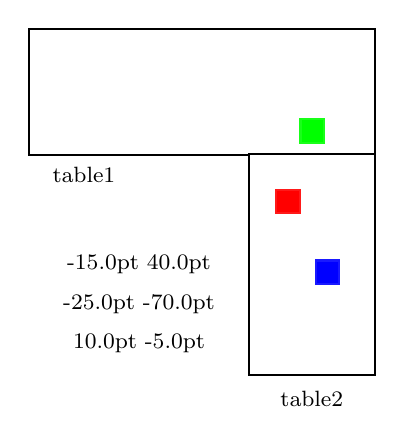
\begin{tikzpicture}
	\coordinate (r) at (-0.15cm, 0.4cm);
	\coordinate (g) at (-0.25cm, -0.7cm);
	\coordinate (b) at (.1cm, -0.05cm);

	\drawtables{}

	%\path let \p1 = (table1.center), \p2=(r) in node[box, fill=red, draw=red!90](red) at (\x1-2*\y2,\y1+2*\x2){};
	\path let \p1 = (table2.center), \p2=(r) in node[box, fill=red, draw=red!90](red) at (\x1+2*\x2,\y1+2*\y2){};
	\path let \p1 = (table1.center), \p2=(g) in node[box, fill=green, draw=green!90](green) at (\x1-2*\y2,\y1+2*\x2){};
	%\path let \p1 = (table2.center), \p2=(g) in node[box, fill=green, draw=green!90](green) at (\x1+2*\x2,\y1+2*\y2){};
	%\path let \p1 = (table1.center), \p2=(b) in node[box, fill=blue, draw=blue!90](blue) at (\x1-2*\y2,\y1+2*\x2){};
	\path let \p1 = (table2.center), \p2=(b) in node[box, fill=blue, draw=blue!90](blue) at (\x1+2*\x2,\y1+2*\y2){};
	
	\path let \p1=(r), \p2=({round(\x1*3.52778)}, {round(\y1*3.52778)}) in node[annot] at(0.2, -1.2){\footnotesize\x2 \y2};
	\path let \p1=(g), \p2=({round(\x1*3.52778)}, {round(\y1*3.52778)}) in node[annot] at(0.2, -1.7){\footnotesize\x2 \y2};
	\path let \p1=(b), \p2=({round(\x1*3.52778)}, {round(\y1*3.52778)}) in node[annot] at(0.2, -2.2){\footnotesize\x2 \y2};


\end{tikzpicture}
\subcaption{Env 022}
\end{subfigure}\hfill
\begin{subfigure}{0.3\textwidth}
\centering
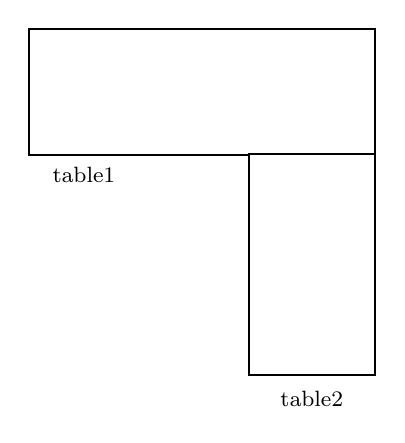
\begin{tikzpicture}
	\coordinate (r) at (0.1cm, -0.6cm);
	\coordinate (g) at (0.1cm, -0.4cm);
	\coordinate (b) at (0.1cm, -0.2cm);

	\drawtables{}

	%\path let \p1 = (table1.center), \p2=(r) in node[box, fill=red, draw=red!90](red) at (\x1-2*\y2,\y1+2*\x2){};
	%\path let \p1 = (table2.center), \p2=(r) in node[box, fill=red, draw=red!90](red) at (\x1+2*\x2,\y1+2*\y2){};
	%\path let \p1 = (table1.center), \p2=(g) in node[box, fill=green, draw=green!90](green) at (\x1-2*\y2,\y1+2*\x2){};
	%\path let \p1 = (table2.center), \p2=(g) in node[box, fill=green, draw=green!90](green) at (\x1+2*\x2,\y1+2*\y2){};
	%\path let \p1 = (table1.center), \p2=(b) in node[box, fill=blue, draw=blue!90](blue) at (\x1-2*\y2,\y1+2*\x2){};
	%\path let \p1 = (table2.center), \p2=(b) in node[box, fill=blue, draw=blue!90](blue) at (\x1+2*\x2,\y1+2*\y2){};
	
	%\path let \p1=(r), \p2=({round(\x1*3.52778)}, {round(\y1*3.52778)}) in node[annot] at(0.2, -1.2){\footnotesize\x2 \y2};
	%\path let \p1=(g), \p2=({round(\x1*3.52778)}, {round(\y1*3.52778)}) in node[annot] at(0.2, -1.7){\footnotesize\x2 \y2};
	%\path let \p1=(b), \p2=({round(\x1*3.52778)}, {round(\y1*3.52778)}) in node[annot] at(0.2, -2.2){\footnotesize\x2 \y2};

\end{tikzpicture}
\subcaption{Env 023}
\end{subfigure}\hfill
\begin{subfigure}{0.3\textwidth}
\centering
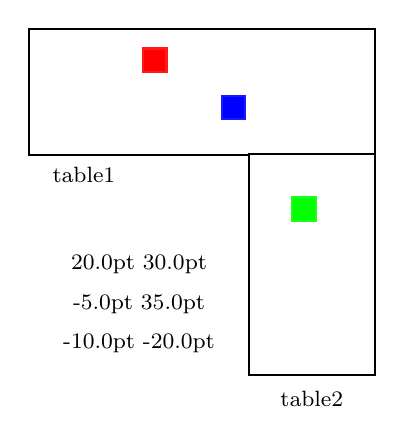
\begin{tikzpicture}
	\coordinate (r) at (0.2cm, 0.3cm);
	\coordinate (g) at (-0.05cm, 0.35cm);
	\coordinate (b) at (-0.1cm, -0.2cm);

	\drawtables{}

	\path let \p1 = (table1.center), \p2=(r) in node[box, fill=red, draw=red!90](red) at (\x1-2*\y2,\y1+2*\x2){};
	%\path let \p1 = (table2.center), \p2=(r) in node[box, fill=red, draw=red!90](red) at (\x1+2*\x2,\y1+2*\y2){};
	%\path let \p1 = (table1.center), \p2=(g) in node[box, fill=green, draw=green!90](green) at (\x1-2*\y2,\y1+2*\x2){};
	\path let \p1 = (table2.center), \p2=(g) in node[box, fill=green, draw=green!90](green) at (\x1+2*\x2,\y1+2*\y2){};
	\path let \p1 = (table1.center), \p2=(b) in node[box, fill=blue, draw=blue!90](blue) at (\x1-2*\y2,\y1+2*\x2){};
	%\path let \p1 = (table2.center), \p2=(b) in node[box, fill=blue, draw=blue!90](blue) at (\x1+2*\x2,\y1+2*\y2){};
	
	\path let \p1=(r), \p2=({round(\x1*3.52778)}, {round(\y1*3.52778)}) in node[annot] at(0.2, -1.2){\footnotesize\x2 \y2};
	\path let \p1=(g), \p2=({round(\x1*3.52778)}, {round(\y1*3.52778)}) in node[annot] at(0.2, -1.7){\footnotesize\x2 \y2};
	\path let \p1=(b), \p2=({round(\x1*3.52778)}, {round(\y1*3.52778)}) in node[annot] at(0.2, -2.2){\footnotesize\x2 \y2};

	
\end{tikzpicture}
\subcaption{Env 024}
\end{subfigure}\\


\begin{subfigure}{0.3\textwidth}
\centering
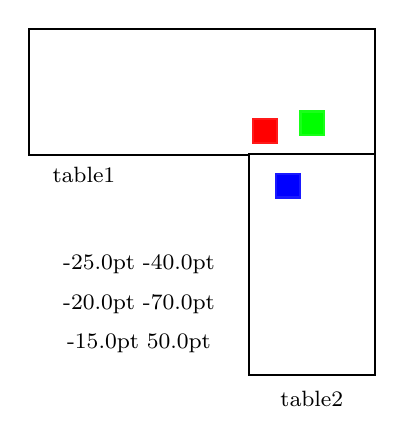
\begin{tikzpicture}
	\coordinate (r) at (-0.25cm, -0.4cm);
	\coordinate (g) at (-0.2cm, -0.7cm);
	\coordinate (b) at (-.15cm, 0.5cm);

	\drawtables{}

	\path let \p1 = (table1.center), \p2=(r) in node[box, fill=red, draw=red!90](red) at (\x1-2*\y2,\y1+2*\x2){};
	%\path let \p1 = (table2.center), \p2=(r) in node[box, fill=red, draw=red!90](red) at (\x1+2*\x2,\y1+2*\y2){};
	\path let \p1 = (table1.center), \p2=(g) in node[box, fill=green, draw=green!90](green) at (\x1-2*\y2,\y1+2*\x2){};
	%\path let \p1 = (table2.center), \p2=(g) in node[box, fill=green, draw=green!90](green) at (\x1+2*\x2,\y1+2*\y2){};
	%\path let \p1 = (table1.center), \p2=(b) in node[box, fill=blue, draw=blue!90](blue) at (\x1-2*\y2,\y1+2*\x2){};
	\path let \p1 = (table2.center), \p2=(b) in node[box, fill=blue, draw=blue!90](blue) at (\x1+2*\x2,\y1+2*\y2){};
	
	\path let \p1=(r), \p2=({round(\x1*3.52778)}, {round(\y1*3.52778)}) in node[annot] at(0.2, -1.2){\footnotesize\x2 \y2};
	\path let \p1=(g), \p2=({round(\x1*3.52778)}, {round(\y1*3.52778)}) in node[annot] at(0.2, -1.7){\footnotesize\x2 \y2};
	\path let \p1=(b), \p2=({round(\x1*3.52778)}, {round(\y1*3.52778)}) in node[annot] at(0.2, -2.2){\footnotesize\x2 \y2};


\end{tikzpicture}
\subcaption{Env 025}
\end{subfigure}\hfill
\begin{subfigure}{0.3\textwidth}
\centering
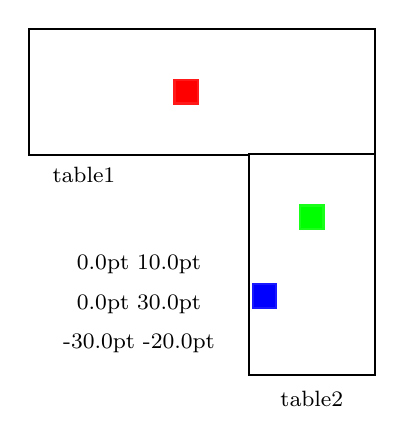
\begin{tikzpicture}
	\coordinate (r) at (0.cm, 0.1cm);
	\coordinate (g) at (0.cm, 0.3cm);
	\coordinate (b) at (-0.3cm, -.2cm);

	\drawtables{}

	\path let \p1 = (table1.center), \p2=(r) in node[box, fill=red, draw=red!90](red) at (\x1-2*\y2,\y1+2*\x2){};
	%\path let \p1 = (table2.center), \p2=(r) in node[box, fill=red, draw=red!90](red) at (\x1+2*\x2,\y1+2*\y2){};
	%\path let \p1 = (table1.center), \p2=(g) in node[box, fill=green, draw=green!90](green) at (\x1-2*\y2,\y1+2*\x2){};
	\path let \p1 = (table2.center), \p2=(g) in node[box, fill=green, draw=green!90](green) at (\x1+2*\x2,\y1+2*\y2){};
	%\path let \p1 = (table1.center), \p2=(b) in node[box, fill=blue, draw=blue!90](blue) at (\x1-2*\y2,\y1+2*\x2){};
	\path let \p1 = (table2.center), \p2=(b) in node[box, fill=blue, draw=blue!90](blue) at (\x1+2*\x2,\y1+2*\y2){};
	
	\path let \p1=(r), \p2=({round(\x1*3.52778)}, {round(\y1*3.52778)}) in node[annot] at(0.2, -1.2){\footnotesize\x2 \y2};
	\path let \p1=(g), \p2=({round(\x1*3.52778)}, {round(\y1*3.52778)}) in node[annot] at(0.2, -1.7){\footnotesize\x2 \y2};
	\path let \p1=(b), \p2=({round(\x1*3.52778)}, {round(\y1*3.52778)}) in node[annot] at(0.2, -2.2){\footnotesize\x2 \y2};

\end{tikzpicture}
\subcaption{Env 026}
\end{subfigure}\hfill
\begin{subfigure}{0.3\textwidth}
\centering
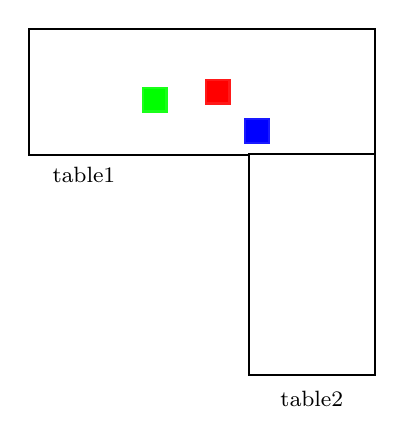
\begin{tikzpicture}
	\coordinate (r) at (0.0cm, -0.1cm);
	\coordinate (g) at (-0.05cm, 0.3cm);
	\coordinate (b) at (-0.25cm, -0.35cm);

	\drawtables{}

	\path let \p1 = (table1.center), \p2=(r) in node[box, fill=red, draw=red!90](red) at (\x1-2*\y2,\y1+2*\x2){};
	%\path let \p1 = (table2.center), \p2=(r) in node[box, fill=red, draw=red!90](red) at (\x1+2*\x2,\y1+2*\y2){};
	\path let \p1 = (table1.center), \p2=(g) in node[box, fill=green, draw=green!90](green) at (\x1-2*\y2,\y1+2*\x2){};
	%\path let \p1 = (table2.center), \p2=(g) in node[box, fill=green, draw=green!90](green) at (\x1+2*\x2,\y1+2*\y2){};
	\path let \p1 = (table1.center), \p2=(b) in node[box, fill=blue, draw=blue!90](blue) at (\x1-2*\y2,\y1+2*\x2){};
	%\path let \p1 = (table2.center), \p2=(b) in node[box, fill=blue, draw=blue!90](blue) at (\x1+2*\x2,\y1+2*\y2){};
	
	%\path let \p1=(r), \p2=({round(\x1*3.52778)}, {round(\y1*3.52778)}) in node[annot] at(0.2, -1.2){\footnotesize\x2 \y2};
	%\path let \p1=(g), \p2=({round(\x1*3.52778)}, {round(\y1*3.52778)}) in node[annot] at(0.2, -1.7){\footnotesize\x2 \y2};
	%\path let \p1=(b), \p2=({round(\x1*3.52778)}, {round(\y1*3.52778)}) in node[annot] at(0.2, -2.2){\footnotesize\x2 \y2};

	
\end{tikzpicture}
\subcaption{Env 027}
\end{subfigure}\\
\end{figure}

\begin{figure}[!h]
\begin{subfigure}{0.3\textwidth}
\centering
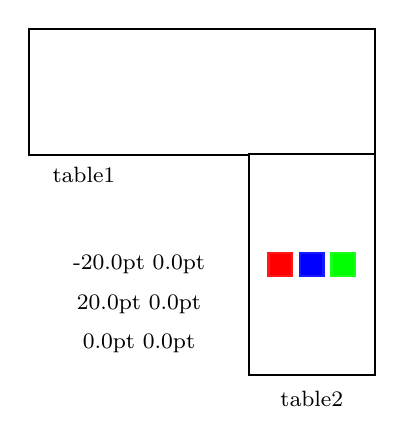
\begin{tikzpicture}
	\coordinate (r) at (-0.2cm, 0cm);
	\coordinate (g) at (0.2cm, 0cm);
	\coordinate (b) at (0cm, 0cm);

	\drawtables{}

	%\path let \p1 = (table1.center), \p2=(r) in node[box, fill=red, draw=red!90](red) at (\x1-2*\y2,\y1+2*\x2){};
	\path let \p1 = (table2.center), \p2=(r) in node[box, fill=red, draw=red!90](red) at (\x1+2*\x2,\y1+2*\y2){};
	%\path let \p1 = (table1.center), \p2=(g) in node[box, fill=green, draw=green!90](green) at (\x1-2*\y2,\y1+2*\x2){};
	\path let \p1 = (table2.center), \p2=(g) in node[box, fill=green, draw=green!90](green) at (\x1+2*\x2,\y1+2*\y2){};
	%\path let \p1 = (table1.center), \p2=(b) in node[box, fill=blue, draw=blue!90](blue) at (\x1-2*\y2,\y1+2*\x2){};
	\path let \p1 = (table2.center), \p2=(b) in node[box, fill=blue, draw=blue!90](blue) at (\x1+2*\x2,\y1+2*\y2){};
	
	\path let \p1=(r), \p2=({round(\x1*3.52778)}, {round(\y1*3.52778)}) in node[annot] at(0.2, -1.2){\footnotesize\x2 \y2};
	\path let \p1=(g), \p2=({round(\x1*3.52778)}, {round(\y1*3.52778)}) in node[annot] at(0.2, -1.7){\footnotesize\x2 \y2};
	\path let \p1=(b), \p2=({round(\x1*3.52778)}, {round(\y1*3.52778)}) in node[annot] at(0.2, -2.2){\footnotesize\x2 \y2};

\end{tikzpicture}
\subcaption{Env 019}
\end{subfigure}\hfill
\begin{subfigure}{0.3\textwidth}
\centering
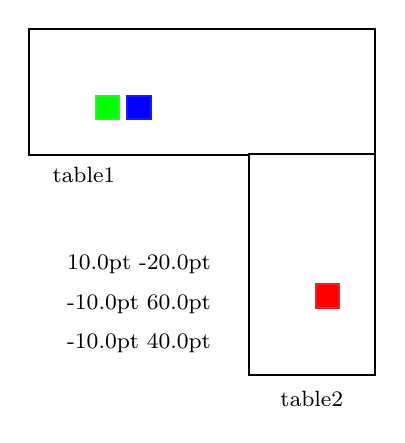
\begin{tikzpicture}
	\coordinate (r) at (0.1cm, -0.2cm);
	\coordinate (g) at (-0.1cm, 0.6cm);
	\coordinate (b) at (-0.1cm, 0.4cm);

	\drawtables{}

	%\path let \p1 = (table1.center), \p2=(r) in node[box, fill=red, draw=red!90](red) at (\x1-2*\y2,\y1+2*\x2){};
	\path let \p1 = (table2.center), \p2=(r) in node[box, fill=red, draw=red!90](red) at (\x1+2*\x2,\y1+2*\y2){};
	\path let \p1 = (table1.center), \p2=(g) in node[box, fill=green, draw=green!90](green) at (\x1-2*\y2,\y1+2*\x2){};
	%\path let \p1 = (table2.center), \p2=(g) in node[box, fill=green, draw=green!90](green) at (\x1+2*\x2,\y1+2*\y2){};
	\path let \p1 = (table1.center), \p2=(b) in node[box, fill=blue, draw=blue!90](blue) at (\x1-2*\y2,\y1+2*\x2){};
	%\path let \p1 = (table2.center), \p2=(b) in node[box, fill=blue, draw=blue!90](blue) at (\x1+2*\x2,\y1+2*\y2){};
	
	\path let \p1=(r), \p2=({round(\x1*3.52778)}, {round(\y1*3.52778)}) in node[annot] at(0.2, -1.2){\footnotesize\x2 \y2};
	\path let \p1=(g), \p2=({round(\x1*3.52778)}, {round(\y1*3.52778)}) in node[annot] at(0.2, -1.7){\footnotesize\x2 \y2};
	\path let \p1=(b), \p2=({round(\x1*3.52778)}, {round(\y1*3.52778)}) in node[annot] at(0.2, -2.2){\footnotesize\x2 \y2};

\end{tikzpicture}
\subcaption{Env 020}
\end{subfigure}\hfill
\begin{subfigure}{0.3\textwidth}
\centering
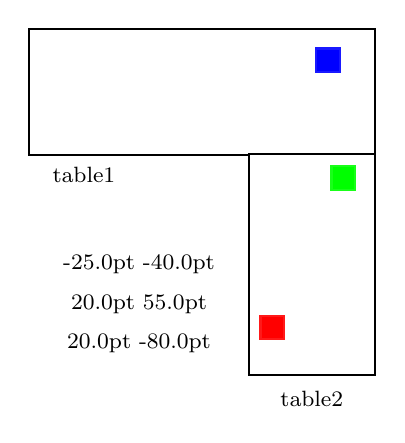
\begin{tikzpicture}
	\coordinate (r) at (-0.25cm, -0.4cm);
	\coordinate (g) at (0.2cm, 0.55cm);
	\coordinate (b) at (0.2cm, -0.8cm);

	\drawtables{}

	%\path let \p1 = (table1.center), \p2=(r) in node[box, fill=red, draw=red!90](red) at (\x1-2*\y2,\y1+2*\x2){};
	\path let \p1 = (table2.center), \p2=(r) in node[box, fill=red, draw=red!90](red) at (\x1+2*\x2,\y1+2*\y2){};
	%\path let \p1 = (table1.center), \p2=(g) in node[box, fill=green, draw=green!90](green) at (\x1-2*\y2,\y1+2*\x2){};
	\path let \p1 = (table2.center), \p2=(g) in node[box, fill=green, draw=green!90](green) at (\x1+2*\x2,\y1+2*\y2){};
	\path let \p1 = (table1.center), \p2=(b) in node[box, fill=blue, draw=blue!90](blue) at (\x1-2*\y2,\y1+2*\x2){};
	%\path let \p1 = (table2.center), \p2=(b) in node[box, fill=blue, draw=blue!90](blue) at (\x1+2*\x2,\y1+2*\y2){};
	
	\path let \p1=(r), \p2=({round(\x1*3.52778)}, {round(\y1*3.52778)}) in node[annot] at(0.2, -1.2){\footnotesize\x2 \y2};
	\path let \p1=(g), \p2=({round(\x1*3.52778)}, {round(\y1*3.52778)}) in node[annot] at(0.2, -1.7){\footnotesize\x2 \y2};
	\path let \p1=(b), \p2=({round(\x1*3.52778)}, {round(\y1*3.52778)}) in node[annot] at(0.2, -2.2){\footnotesize\x2 \y2};

	
\end{tikzpicture}
\subcaption{Env 021}
\end{subfigure}\\

\begin{subfigure}{0.3\textwidth}
\centering
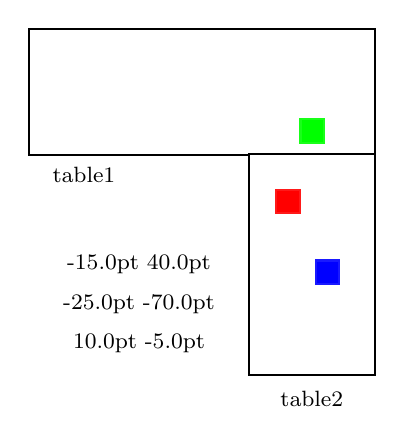
\begin{tikzpicture}
	\coordinate (r) at (-0.15cm, 0.4cm);
	\coordinate (g) at (-0.25cm, -0.7cm);
	\coordinate (b) at (.1cm, -0.05cm);

	\drawtables{}

	%\path let \p1 = (table1.center), \p2=(r) in node[box, fill=red, draw=red!90](red) at (\x1-2*\y2,\y1+2*\x2){};
	\path let \p1 = (table2.center), \p2=(r) in node[box, fill=red, draw=red!90](red) at (\x1+2*\x2,\y1+2*\y2){};
	\path let \p1 = (table1.center), \p2=(g) in node[box, fill=green, draw=green!90](green) at (\x1-2*\y2,\y1+2*\x2){};
	%\path let \p1 = (table2.center), \p2=(g) in node[box, fill=green, draw=green!90](green) at (\x1+2*\x2,\y1+2*\y2){};
	%\path let \p1 = (table1.center), \p2=(b) in node[box, fill=blue, draw=blue!90](blue) at (\x1-2*\y2,\y1+2*\x2){};
	\path let \p1 = (table2.center), \p2=(b) in node[box, fill=blue, draw=blue!90](blue) at (\x1+2*\x2,\y1+2*\y2){};
	
	\path let \p1=(r), \p2=({round(\x1*3.52778)}, {round(\y1*3.52778)}) in node[annot] at(0.2, -1.2){\footnotesize\x2 \y2};
	\path let \p1=(g), \p2=({round(\x1*3.52778)}, {round(\y1*3.52778)}) in node[annot] at(0.2, -1.7){\footnotesize\x2 \y2};
	\path let \p1=(b), \p2=({round(\x1*3.52778)}, {round(\y1*3.52778)}) in node[annot] at(0.2, -2.2){\footnotesize\x2 \y2};


\end{tikzpicture}
\subcaption{Env 022}
\end{subfigure}\hfill
\begin{subfigure}{0.3\textwidth}
\centering
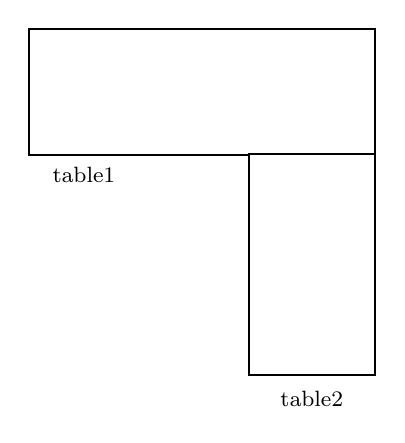
\begin{tikzpicture}
	\coordinate (r) at (0.1cm, -0.6cm);
	\coordinate (g) at (0.1cm, -0.4cm);
	\coordinate (b) at (0.1cm, -0.2cm);

	\drawtables{}

	%\path let \p1 = (table1.center), \p2=(r) in node[box, fill=red, draw=red!90](red) at (\x1-2*\y2,\y1+2*\x2){};
	%\path let \p1 = (table2.center), \p2=(r) in node[box, fill=red, draw=red!90](red) at (\x1+2*\x2,\y1+2*\y2){};
	%\path let \p1 = (table1.center), \p2=(g) in node[box, fill=green, draw=green!90](green) at (\x1-2*\y2,\y1+2*\x2){};
	%\path let \p1 = (table2.center), \p2=(g) in node[box, fill=green, draw=green!90](green) at (\x1+2*\x2,\y1+2*\y2){};
	%\path let \p1 = (table1.center), \p2=(b) in node[box, fill=blue, draw=blue!90](blue) at (\x1-2*\y2,\y1+2*\x2){};
	%\path let \p1 = (table2.center), \p2=(b) in node[box, fill=blue, draw=blue!90](blue) at (\x1+2*\x2,\y1+2*\y2){};
	
	%\path let \p1=(r), \p2=({round(\x1*3.52778)}, {round(\y1*3.52778)}) in node[annot] at(0.2, -1.2){\footnotesize\x2 \y2};
	%\path let \p1=(g), \p2=({round(\x1*3.52778)}, {round(\y1*3.52778)}) in node[annot] at(0.2, -1.7){\footnotesize\x2 \y2};
	%\path let \p1=(b), \p2=({round(\x1*3.52778)}, {round(\y1*3.52778)}) in node[annot] at(0.2, -2.2){\footnotesize\x2 \y2};

\end{tikzpicture}
\subcaption{Env 023}
\end{subfigure}\hfill
\begin{subfigure}{0.3\textwidth}
\centering
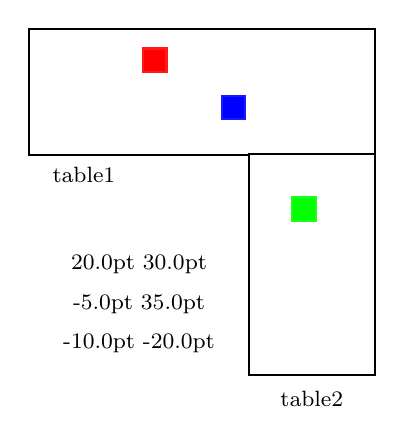
\begin{tikzpicture}
	\coordinate (r) at (0.2cm, 0.3cm);
	\coordinate (g) at (-0.05cm, 0.35cm);
	\coordinate (b) at (-0.1cm, -0.2cm);

	\drawtables{}

	\path let \p1 = (table1.center), \p2=(r) in node[box, fill=red, draw=red!90](red) at (\x1-2*\y2,\y1+2*\x2){};
	%\path let \p1 = (table2.center), \p2=(r) in node[box, fill=red, draw=red!90](red) at (\x1+2*\x2,\y1+2*\y2){};
	%\path let \p1 = (table1.center), \p2=(g) in node[box, fill=green, draw=green!90](green) at (\x1-2*\y2,\y1+2*\x2){};
	\path let \p1 = (table2.center), \p2=(g) in node[box, fill=green, draw=green!90](green) at (\x1+2*\x2,\y1+2*\y2){};
	\path let \p1 = (table1.center), \p2=(b) in node[box, fill=blue, draw=blue!90](blue) at (\x1-2*\y2,\y1+2*\x2){};
	%\path let \p1 = (table2.center), \p2=(b) in node[box, fill=blue, draw=blue!90](blue) at (\x1+2*\x2,\y1+2*\y2){};
	
	\path let \p1=(r), \p2=({round(\x1*3.52778)}, {round(\y1*3.52778)}) in node[annot] at(0.2, -1.2){\footnotesize\x2 \y2};
	\path let \p1=(g), \p2=({round(\x1*3.52778)}, {round(\y1*3.52778)}) in node[annot] at(0.2, -1.7){\footnotesize\x2 \y2};
	\path let \p1=(b), \p2=({round(\x1*3.52778)}, {round(\y1*3.52778)}) in node[annot] at(0.2, -2.2){\footnotesize\x2 \y2};

	
\end{tikzpicture}
\subcaption{Env 024}
\end{subfigure}\\


\begin{subfigure}{0.3\textwidth}
\centering
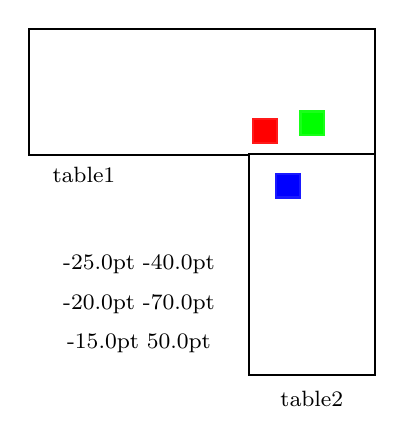
\begin{tikzpicture}
	\coordinate (r) at (-0.25cm, -0.4cm);
	\coordinate (g) at (-0.2cm, -0.7cm);
	\coordinate (b) at (-.15cm, 0.5cm);

	\drawtables{}

	\path let \p1 = (table1.center), \p2=(r) in node[box, fill=red, draw=red!90](red) at (\x1-2*\y2,\y1+2*\x2){};
	%\path let \p1 = (table2.center), \p2=(r) in node[box, fill=red, draw=red!90](red) at (\x1+2*\x2,\y1+2*\y2){};
	\path let \p1 = (table1.center), \p2=(g) in node[box, fill=green, draw=green!90](green) at (\x1-2*\y2,\y1+2*\x2){};
	%\path let \p1 = (table2.center), \p2=(g) in node[box, fill=green, draw=green!90](green) at (\x1+2*\x2,\y1+2*\y2){};
	%\path let \p1 = (table1.center), \p2=(b) in node[box, fill=blue, draw=blue!90](blue) at (\x1-2*\y2,\y1+2*\x2){};
	\path let \p1 = (table2.center), \p2=(b) in node[box, fill=blue, draw=blue!90](blue) at (\x1+2*\x2,\y1+2*\y2){};
	
	\path let \p1=(r), \p2=({round(\x1*3.52778)}, {round(\y1*3.52778)}) in node[annot] at(0.2, -1.2){\footnotesize\x2 \y2};
	\path let \p1=(g), \p2=({round(\x1*3.52778)}, {round(\y1*3.52778)}) in node[annot] at(0.2, -1.7){\footnotesize\x2 \y2};
	\path let \p1=(b), \p2=({round(\x1*3.52778)}, {round(\y1*3.52778)}) in node[annot] at(0.2, -2.2){\footnotesize\x2 \y2};


\end{tikzpicture}
\subcaption{Env 025}
\end{subfigure}\hfill
\begin{subfigure}{0.3\textwidth}
\centering
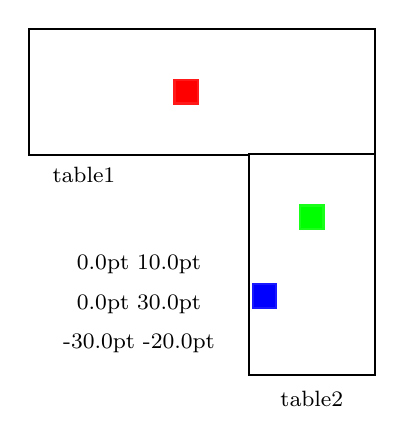
\begin{tikzpicture}
	\coordinate (r) at (0.cm, 0.1cm);
	\coordinate (g) at (0.cm, 0.3cm);
	\coordinate (b) at (-0.3cm, -.2cm);

	\drawtables{}

	\path let \p1 = (table1.center), \p2=(r) in node[box, fill=red, draw=red!90](red) at (\x1-2*\y2,\y1+2*\x2){};
	%\path let \p1 = (table2.center), \p2=(r) in node[box, fill=red, draw=red!90](red) at (\x1+2*\x2,\y1+2*\y2){};
	%\path let \p1 = (table1.center), \p2=(g) in node[box, fill=green, draw=green!90](green) at (\x1-2*\y2,\y1+2*\x2){};
	\path let \p1 = (table2.center), \p2=(g) in node[box, fill=green, draw=green!90](green) at (\x1+2*\x2,\y1+2*\y2){};
	%\path let \p1 = (table1.center), \p2=(b) in node[box, fill=blue, draw=blue!90](blue) at (\x1-2*\y2,\y1+2*\x2){};
	\path let \p1 = (table2.center), \p2=(b) in node[box, fill=blue, draw=blue!90](blue) at (\x1+2*\x2,\y1+2*\y2){};
	
	\path let \p1=(r), \p2=({round(\x1*3.52778)}, {round(\y1*3.52778)}) in node[annot] at(0.2, -1.2){\footnotesize\x2 \y2};
	\path let \p1=(g), \p2=({round(\x1*3.52778)}, {round(\y1*3.52778)}) in node[annot] at(0.2, -1.7){\footnotesize\x2 \y2};
	\path let \p1=(b), \p2=({round(\x1*3.52778)}, {round(\y1*3.52778)}) in node[annot] at(0.2, -2.2){\footnotesize\x2 \y2};

\end{tikzpicture}
\subcaption{Env 026}
\end{subfigure}\hfill
\begin{subfigure}{0.3\textwidth}
\centering
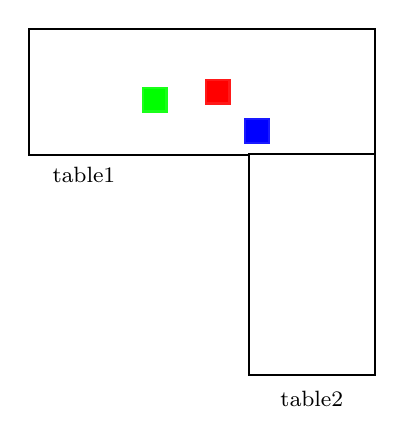
\begin{tikzpicture}
	\coordinate (r) at (0.0cm, -0.1cm);
	\coordinate (g) at (-0.05cm, 0.3cm);
	\coordinate (b) at (-0.25cm, -0.35cm);

	\drawtables{}

	\path let \p1 = (table1.center), \p2=(r) in node[box, fill=red, draw=red!90](red) at (\x1-2*\y2,\y1+2*\x2){};
	%\path let \p1 = (table2.center), \p2=(r) in node[box, fill=red, draw=red!90](red) at (\x1+2*\x2,\y1+2*\y2){};
	\path let \p1 = (table1.center), \p2=(g) in node[box, fill=green, draw=green!90](green) at (\x1-2*\y2,\y1+2*\x2){};
	%\path let \p1 = (table2.center), \p2=(g) in node[box, fill=green, draw=green!90](green) at (\x1+2*\x2,\y1+2*\y2){};
	\path let \p1 = (table1.center), \p2=(b) in node[box, fill=blue, draw=blue!90](blue) at (\x1-2*\y2,\y1+2*\x2){};
	%\path let \p1 = (table2.center), \p2=(b) in node[box, fill=blue, draw=blue!90](blue) at (\x1+2*\x2,\y1+2*\y2){};
	
	%\path let \p1=(r), \p2=({round(\x1*3.52778)}, {round(\y1*3.52778)}) in node[annot] at(0.2, -1.2){\footnotesize\x2 \y2};
	%\path let \p1=(g), \p2=({round(\x1*3.52778)}, {round(\y1*3.52778)}) in node[annot] at(0.2, -1.7){\footnotesize\x2 \y2};
	%\path let \p1=(b), \p2=({round(\x1*3.52778)}, {round(\y1*3.52778)}) in node[annot] at(0.2, -2.2){\footnotesize\x2 \y2};

	
\end{tikzpicture}
\subcaption{Env 027}
\end{subfigure}\\
\end{figure}

\begin{figure}[!h]
\begin{subfigure}{0.3\textwidth}
\centering
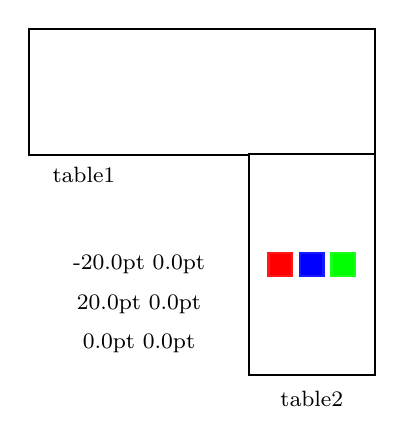
\begin{tikzpicture}
	\coordinate (r) at (-0.2cm, 0cm);
	\coordinate (g) at (0.2cm, 0cm);
	\coordinate (b) at (0cm, 0cm);

	\drawtables{}

	%\path let \p1 = (table1.center), \p2=(r) in node[box, fill=red, draw=red!90](red) at (\x1-2*\y2,\y1+2*\x2){};
	\path let \p1 = (table2.center), \p2=(r) in node[box, fill=red, draw=red!90](red) at (\x1+2*\x2,\y1+2*\y2){};
	%\path let \p1 = (table1.center), \p2=(g) in node[box, fill=green, draw=green!90](green) at (\x1-2*\y2,\y1+2*\x2){};
	\path let \p1 = (table2.center), \p2=(g) in node[box, fill=green, draw=green!90](green) at (\x1+2*\x2,\y1+2*\y2){};
	%\path let \p1 = (table1.center), \p2=(b) in node[box, fill=blue, draw=blue!90](blue) at (\x1-2*\y2,\y1+2*\x2){};
	\path let \p1 = (table2.center), \p2=(b) in node[box, fill=blue, draw=blue!90](blue) at (\x1+2*\x2,\y1+2*\y2){};
	
	\path let \p1=(r), \p2=({round(\x1*3.52778)}, {round(\y1*3.52778)}) in node[annot] at(0.2, -1.2){\footnotesize\x2 \y2};
	\path let \p1=(g), \p2=({round(\x1*3.52778)}, {round(\y1*3.52778)}) in node[annot] at(0.2, -1.7){\footnotesize\x2 \y2};
	\path let \p1=(b), \p2=({round(\x1*3.52778)}, {round(\y1*3.52778)}) in node[annot] at(0.2, -2.2){\footnotesize\x2 \y2};

\end{tikzpicture}
\subcaption{Env 019}
\end{subfigure}\hfill
\begin{subfigure}{0.3\textwidth}
\centering
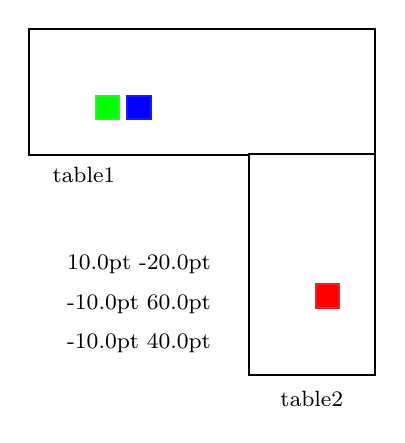
\begin{tikzpicture}
	\coordinate (r) at (0.1cm, -0.2cm);
	\coordinate (g) at (-0.1cm, 0.6cm);
	\coordinate (b) at (-0.1cm, 0.4cm);

	\drawtables{}

	%\path let \p1 = (table1.center), \p2=(r) in node[box, fill=red, draw=red!90](red) at (\x1-2*\y2,\y1+2*\x2){};
	\path let \p1 = (table2.center), \p2=(r) in node[box, fill=red, draw=red!90](red) at (\x1+2*\x2,\y1+2*\y2){};
	\path let \p1 = (table1.center), \p2=(g) in node[box, fill=green, draw=green!90](green) at (\x1-2*\y2,\y1+2*\x2){};
	%\path let \p1 = (table2.center), \p2=(g) in node[box, fill=green, draw=green!90](green) at (\x1+2*\x2,\y1+2*\y2){};
	\path let \p1 = (table1.center), \p2=(b) in node[box, fill=blue, draw=blue!90](blue) at (\x1-2*\y2,\y1+2*\x2){};
	%\path let \p1 = (table2.center), \p2=(b) in node[box, fill=blue, draw=blue!90](blue) at (\x1+2*\x2,\y1+2*\y2){};
	
	\path let \p1=(r), \p2=({round(\x1*3.52778)}, {round(\y1*3.52778)}) in node[annot] at(0.2, -1.2){\footnotesize\x2 \y2};
	\path let \p1=(g), \p2=({round(\x1*3.52778)}, {round(\y1*3.52778)}) in node[annot] at(0.2, -1.7){\footnotesize\x2 \y2};
	\path let \p1=(b), \p2=({round(\x1*3.52778)}, {round(\y1*3.52778)}) in node[annot] at(0.2, -2.2){\footnotesize\x2 \y2};

\end{tikzpicture}
\subcaption{Env 020}
\end{subfigure}\hfill
\begin{subfigure}{0.3\textwidth}
\centering
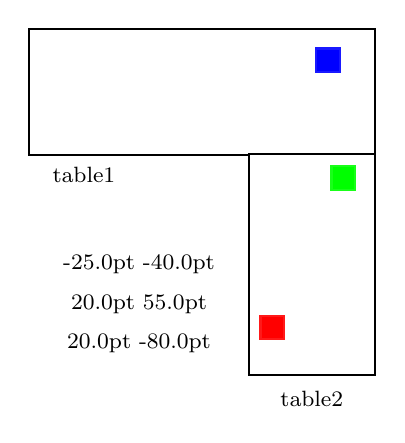
\begin{tikzpicture}
	\coordinate (r) at (-0.25cm, -0.4cm);
	\coordinate (g) at (0.2cm, 0.55cm);
	\coordinate (b) at (0.2cm, -0.8cm);

	\drawtables{}

	%\path let \p1 = (table1.center), \p2=(r) in node[box, fill=red, draw=red!90](red) at (\x1-2*\y2,\y1+2*\x2){};
	\path let \p1 = (table2.center), \p2=(r) in node[box, fill=red, draw=red!90](red) at (\x1+2*\x2,\y1+2*\y2){};
	%\path let \p1 = (table1.center), \p2=(g) in node[box, fill=green, draw=green!90](green) at (\x1-2*\y2,\y1+2*\x2){};
	\path let \p1 = (table2.center), \p2=(g) in node[box, fill=green, draw=green!90](green) at (\x1+2*\x2,\y1+2*\y2){};
	\path let \p1 = (table1.center), \p2=(b) in node[box, fill=blue, draw=blue!90](blue) at (\x1-2*\y2,\y1+2*\x2){};
	%\path let \p1 = (table2.center), \p2=(b) in node[box, fill=blue, draw=blue!90](blue) at (\x1+2*\x2,\y1+2*\y2){};
	
	\path let \p1=(r), \p2=({round(\x1*3.52778)}, {round(\y1*3.52778)}) in node[annot] at(0.2, -1.2){\footnotesize\x2 \y2};
	\path let \p1=(g), \p2=({round(\x1*3.52778)}, {round(\y1*3.52778)}) in node[annot] at(0.2, -1.7){\footnotesize\x2 \y2};
	\path let \p1=(b), \p2=({round(\x1*3.52778)}, {round(\y1*3.52778)}) in node[annot] at(0.2, -2.2){\footnotesize\x2 \y2};

	
\end{tikzpicture}
\subcaption{Env 021}
\end{subfigure}\\

\begin{subfigure}{0.3\textwidth}
\centering
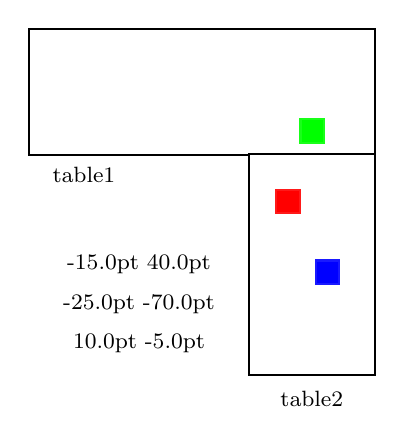
\begin{tikzpicture}
	\coordinate (r) at (-0.15cm, 0.4cm);
	\coordinate (g) at (-0.25cm, -0.7cm);
	\coordinate (b) at (.1cm, -0.05cm);

	\drawtables{}

	%\path let \p1 = (table1.center), \p2=(r) in node[box, fill=red, draw=red!90](red) at (\x1-2*\y2,\y1+2*\x2){};
	\path let \p1 = (table2.center), \p2=(r) in node[box, fill=red, draw=red!90](red) at (\x1+2*\x2,\y1+2*\y2){};
	\path let \p1 = (table1.center), \p2=(g) in node[box, fill=green, draw=green!90](green) at (\x1-2*\y2,\y1+2*\x2){};
	%\path let \p1 = (table2.center), \p2=(g) in node[box, fill=green, draw=green!90](green) at (\x1+2*\x2,\y1+2*\y2){};
	%\path let \p1 = (table1.center), \p2=(b) in node[box, fill=blue, draw=blue!90](blue) at (\x1-2*\y2,\y1+2*\x2){};
	\path let \p1 = (table2.center), \p2=(b) in node[box, fill=blue, draw=blue!90](blue) at (\x1+2*\x2,\y1+2*\y2){};
	
	\path let \p1=(r), \p2=({round(\x1*3.52778)}, {round(\y1*3.52778)}) in node[annot] at(0.2, -1.2){\footnotesize\x2 \y2};
	\path let \p1=(g), \p2=({round(\x1*3.52778)}, {round(\y1*3.52778)}) in node[annot] at(0.2, -1.7){\footnotesize\x2 \y2};
	\path let \p1=(b), \p2=({round(\x1*3.52778)}, {round(\y1*3.52778)}) in node[annot] at(0.2, -2.2){\footnotesize\x2 \y2};


\end{tikzpicture}
\subcaption{Env 022}
\end{subfigure}\hfill
\begin{subfigure}{0.3\textwidth}
\centering
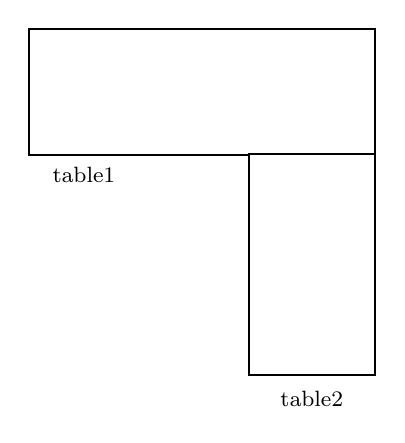
\begin{tikzpicture}
	\coordinate (r) at (0.1cm, -0.6cm);
	\coordinate (g) at (0.1cm, -0.4cm);
	\coordinate (b) at (0.1cm, -0.2cm);

	\drawtables{}

	%\path let \p1 = (table1.center), \p2=(r) in node[box, fill=red, draw=red!90](red) at (\x1-2*\y2,\y1+2*\x2){};
	%\path let \p1 = (table2.center), \p2=(r) in node[box, fill=red, draw=red!90](red) at (\x1+2*\x2,\y1+2*\y2){};
	%\path let \p1 = (table1.center), \p2=(g) in node[box, fill=green, draw=green!90](green) at (\x1-2*\y2,\y1+2*\x2){};
	%\path let \p1 = (table2.center), \p2=(g) in node[box, fill=green, draw=green!90](green) at (\x1+2*\x2,\y1+2*\y2){};
	%\path let \p1 = (table1.center), \p2=(b) in node[box, fill=blue, draw=blue!90](blue) at (\x1-2*\y2,\y1+2*\x2){};
	%\path let \p1 = (table2.center), \p2=(b) in node[box, fill=blue, draw=blue!90](blue) at (\x1+2*\x2,\y1+2*\y2){};
	
	%\path let \p1=(r), \p2=({round(\x1*3.52778)}, {round(\y1*3.52778)}) in node[annot] at(0.2, -1.2){\footnotesize\x2 \y2};
	%\path let \p1=(g), \p2=({round(\x1*3.52778)}, {round(\y1*3.52778)}) in node[annot] at(0.2, -1.7){\footnotesize\x2 \y2};
	%\path let \p1=(b), \p2=({round(\x1*3.52778)}, {round(\y1*3.52778)}) in node[annot] at(0.2, -2.2){\footnotesize\x2 \y2};

\end{tikzpicture}
\subcaption{Env 023}
\end{subfigure}\hfill
\begin{subfigure}{0.3\textwidth}
\centering
\begin{tikzpicture}
	\coordinate (r) at (0.2cm, 0.3cm);
	\coordinate (g) at (-0.05cm, 0.35cm);
	\coordinate (b) at (-0.1cm, -0.2cm);

	\drawtables{}

	\path let \p1 = (table1.center), \p2=(r) in node[box, fill=red, draw=red!90](red) at (\x1-2*\y2,\y1+2*\x2){};
	%\path let \p1 = (table2.center), \p2=(r) in node[box, fill=red, draw=red!90](red) at (\x1+2*\x2,\y1+2*\y2){};
	%\path let \p1 = (table1.center), \p2=(g) in node[box, fill=green, draw=green!90](green) at (\x1-2*\y2,\y1+2*\x2){};
	\path let \p1 = (table2.center), \p2=(g) in node[box, fill=green, draw=green!90](green) at (\x1+2*\x2,\y1+2*\y2){};
	\path let \p1 = (table1.center), \p2=(b) in node[box, fill=blue, draw=blue!90](blue) at (\x1-2*\y2,\y1+2*\x2){};
	%\path let \p1 = (table2.center), \p2=(b) in node[box, fill=blue, draw=blue!90](blue) at (\x1+2*\x2,\y1+2*\y2){};
	
	\path let \p1=(r), \p2=({round(\x1*3.52778)}, {round(\y1*3.52778)}) in node[annot] at(0.2, -1.2){\footnotesize\x2 \y2};
	\path let \p1=(g), \p2=({round(\x1*3.52778)}, {round(\y1*3.52778)}) in node[annot] at(0.2, -1.7){\footnotesize\x2 \y2};
	\path let \p1=(b), \p2=({round(\x1*3.52778)}, {round(\y1*3.52778)}) in node[annot] at(0.2, -2.2){\footnotesize\x2 \y2};

	
\end{tikzpicture}
\subcaption{Env 024}
\end{subfigure}\\


\begin{subfigure}{0.3\textwidth}
\centering
\begin{tikzpicture}
	\coordinate (r) at (-0.25cm, -0.4cm);
	\coordinate (g) at (-0.2cm, -0.7cm);
	\coordinate (b) at (-.15cm, 0.5cm);

	\drawtables{}

	\path let \p1 = (table1.center), \p2=(r) in node[box, fill=red, draw=red!90](red) at (\x1-2*\y2,\y1+2*\x2){};
	%\path let \p1 = (table2.center), \p2=(r) in node[box, fill=red, draw=red!90](red) at (\x1+2*\x2,\y1+2*\y2){};
	\path let \p1 = (table1.center), \p2=(g) in node[box, fill=green, draw=green!90](green) at (\x1-2*\y2,\y1+2*\x2){};
	%\path let \p1 = (table2.center), \p2=(g) in node[box, fill=green, draw=green!90](green) at (\x1+2*\x2,\y1+2*\y2){};
	%\path let \p1 = (table1.center), \p2=(b) in node[box, fill=blue, draw=blue!90](blue) at (\x1-2*\y2,\y1+2*\x2){};
	\path let \p1 = (table2.center), \p2=(b) in node[box, fill=blue, draw=blue!90](blue) at (\x1+2*\x2,\y1+2*\y2){};
	
	\path let \p1=(r), \p2=({round(\x1*3.52778)}, {round(\y1*3.52778)}) in node[annot] at(0.2, -1.2){\footnotesize\x2 \y2};
	\path let \p1=(g), \p2=({round(\x1*3.52778)}, {round(\y1*3.52778)}) in node[annot] at(0.2, -1.7){\footnotesize\x2 \y2};
	\path let \p1=(b), \p2=({round(\x1*3.52778)}, {round(\y1*3.52778)}) in node[annot] at(0.2, -2.2){\footnotesize\x2 \y2};


\end{tikzpicture}
\subcaption{Env 025}
\end{subfigure}\hfill
\begin{subfigure}{0.3\textwidth}
\centering
\begin{tikzpicture}
	\coordinate (r) at (0.cm, 0.1cm);
	\coordinate (g) at (0.cm, 0.3cm);
	\coordinate (b) at (-0.3cm, -.2cm);

	\drawtables{}

	\path let \p1 = (table1.center), \p2=(r) in node[box, fill=red, draw=red!90](red) at (\x1-2*\y2,\y1+2*\x2){};
	%\path let \p1 = (table2.center), \p2=(r) in node[box, fill=red, draw=red!90](red) at (\x1+2*\x2,\y1+2*\y2){};
	%\path let \p1 = (table1.center), \p2=(g) in node[box, fill=green, draw=green!90](green) at (\x1-2*\y2,\y1+2*\x2){};
	\path let \p1 = (table2.center), \p2=(g) in node[box, fill=green, draw=green!90](green) at (\x1+2*\x2,\y1+2*\y2){};
	%\path let \p1 = (table1.center), \p2=(b) in node[box, fill=blue, draw=blue!90](blue) at (\x1-2*\y2,\y1+2*\x2){};
	\path let \p1 = (table2.center), \p2=(b) in node[box, fill=blue, draw=blue!90](blue) at (\x1+2*\x2,\y1+2*\y2){};
	
	\path let \p1=(r), \p2=({round(\x1*3.52778)}, {round(\y1*3.52778)}) in node[annot] at(0.2, -1.2){\footnotesize\x2 \y2};
	\path let \p1=(g), \p2=({round(\x1*3.52778)}, {round(\y1*3.52778)}) in node[annot] at(0.2, -1.7){\footnotesize\x2 \y2};
	\path let \p1=(b), \p2=({round(\x1*3.52778)}, {round(\y1*3.52778)}) in node[annot] at(0.2, -2.2){\footnotesize\x2 \y2};

\end{tikzpicture}
\subcaption{Env 026}
\end{subfigure}\hfill
\begin{subfigure}{0.3\textwidth}
\centering
\begin{tikzpicture}
	\coordinate (r) at (0.0cm, -0.1cm);
	\coordinate (g) at (-0.05cm, 0.3cm);
	\coordinate (b) at (-0.25cm, -0.35cm);

	\drawtables{}

	\path let \p1 = (table1.center), \p2=(r) in node[box, fill=red, draw=red!90](red) at (\x1-2*\y2,\y1+2*\x2){};
	%\path let \p1 = (table2.center), \p2=(r) in node[box, fill=red, draw=red!90](red) at (\x1+2*\x2,\y1+2*\y2){};
	\path let \p1 = (table1.center), \p2=(g) in node[box, fill=green, draw=green!90](green) at (\x1-2*\y2,\y1+2*\x2){};
	%\path let \p1 = (table2.center), \p2=(g) in node[box, fill=green, draw=green!90](green) at (\x1+2*\x2,\y1+2*\y2){};
	\path let \p1 = (table1.center), \p2=(b) in node[box, fill=blue, draw=blue!90](blue) at (\x1-2*\y2,\y1+2*\x2){};
	%\path let \p1 = (table2.center), \p2=(b) in node[box, fill=blue, draw=blue!90](blue) at (\x1+2*\x2,\y1+2*\y2){};
	
	%\path let \p1=(r), \p2=({round(\x1*3.52778)}, {round(\y1*3.52778)}) in node[annot] at(0.2, -1.2){\footnotesize\x2 \y2};
	%\path let \p1=(g), \p2=({round(\x1*3.52778)}, {round(\y1*3.52778)}) in node[annot] at(0.2, -1.7){\footnotesize\x2 \y2};
	%\path let \p1=(b), \p2=({round(\x1*3.52778)}, {round(\y1*3.52778)}) in node[annot] at(0.2, -2.2){\footnotesize\x2 \y2};

	
\end{tikzpicture}
\subcaption{Env 027}
\end{subfigure}\\
\end{figure}

\begin{figure}[!h]
\begin{subfigure}{0.3\textwidth}
\centering
\begin{tikzpicture}
	\coordinate (r) at (-0.2cm, 0cm);
	\coordinate (g) at (0.2cm, 0cm);
	\coordinate (b) at (0cm, 0cm);

	\drawtables{}

	%\path let \p1 = (table1.center), \p2=(r) in node[box, fill=red, draw=red!90](red) at (\x1-2*\y2,\y1+2*\x2){};
	\path let \p1 = (table2.center), \p2=(r) in node[box, fill=red, draw=red!90](red) at (\x1+2*\x2,\y1+2*\y2){};
	%\path let \p1 = (table1.center), \p2=(g) in node[box, fill=green, draw=green!90](green) at (\x1-2*\y2,\y1+2*\x2){};
	\path let \p1 = (table2.center), \p2=(g) in node[box, fill=green, draw=green!90](green) at (\x1+2*\x2,\y1+2*\y2){};
	%\path let \p1 = (table1.center), \p2=(b) in node[box, fill=blue, draw=blue!90](blue) at (\x1-2*\y2,\y1+2*\x2){};
	\path let \p1 = (table2.center), \p2=(b) in node[box, fill=blue, draw=blue!90](blue) at (\x1+2*\x2,\y1+2*\y2){};
	
	\path let \p1=(r), \p2=({round(\x1*3.52778)}, {round(\y1*3.52778)}) in node[annot] at(0.2, -1.2){\footnotesize\x2 \y2};
	\path let \p1=(g), \p2=({round(\x1*3.52778)}, {round(\y1*3.52778)}) in node[annot] at(0.2, -1.7){\footnotesize\x2 \y2};
	\path let \p1=(b), \p2=({round(\x1*3.52778)}, {round(\y1*3.52778)}) in node[annot] at(0.2, -2.2){\footnotesize\x2 \y2};

\end{tikzpicture}
\subcaption{Env 019}
\end{subfigure}\hfill
\begin{subfigure}{0.3\textwidth}
\centering
\begin{tikzpicture}
	\coordinate (r) at (0.1cm, -0.2cm);
	\coordinate (g) at (-0.1cm, 0.6cm);
	\coordinate (b) at (-0.1cm, 0.4cm);

	\drawtables{}

	%\path let \p1 = (table1.center), \p2=(r) in node[box, fill=red, draw=red!90](red) at (\x1-2*\y2,\y1+2*\x2){};
	\path let \p1 = (table2.center), \p2=(r) in node[box, fill=red, draw=red!90](red) at (\x1+2*\x2,\y1+2*\y2){};
	\path let \p1 = (table1.center), \p2=(g) in node[box, fill=green, draw=green!90](green) at (\x1-2*\y2,\y1+2*\x2){};
	%\path let \p1 = (table2.center), \p2=(g) in node[box, fill=green, draw=green!90](green) at (\x1+2*\x2,\y1+2*\y2){};
	\path let \p1 = (table1.center), \p2=(b) in node[box, fill=blue, draw=blue!90](blue) at (\x1-2*\y2,\y1+2*\x2){};
	%\path let \p1 = (table2.center), \p2=(b) in node[box, fill=blue, draw=blue!90](blue) at (\x1+2*\x2,\y1+2*\y2){};
	
	\path let \p1=(r), \p2=({round(\x1*3.52778)}, {round(\y1*3.52778)}) in node[annot] at(0.2, -1.2){\footnotesize\x2 \y2};
	\path let \p1=(g), \p2=({round(\x1*3.52778)}, {round(\y1*3.52778)}) in node[annot] at(0.2, -1.7){\footnotesize\x2 \y2};
	\path let \p1=(b), \p2=({round(\x1*3.52778)}, {round(\y1*3.52778)}) in node[annot] at(0.2, -2.2){\footnotesize\x2 \y2};

\end{tikzpicture}
\subcaption{Env 020}
\end{subfigure}\hfill
\begin{subfigure}{0.3\textwidth}
\centering
\begin{tikzpicture}
	\coordinate (r) at (-0.25cm, -0.4cm);
	\coordinate (g) at (0.2cm, 0.55cm);
	\coordinate (b) at (0.2cm, -0.8cm);

	\drawtables{}

	%\path let \p1 = (table1.center), \p2=(r) in node[box, fill=red, draw=red!90](red) at (\x1-2*\y2,\y1+2*\x2){};
	\path let \p1 = (table2.center), \p2=(r) in node[box, fill=red, draw=red!90](red) at (\x1+2*\x2,\y1+2*\y2){};
	%\path let \p1 = (table1.center), \p2=(g) in node[box, fill=green, draw=green!90](green) at (\x1-2*\y2,\y1+2*\x2){};
	\path let \p1 = (table2.center), \p2=(g) in node[box, fill=green, draw=green!90](green) at (\x1+2*\x2,\y1+2*\y2){};
	\path let \p1 = (table1.center), \p2=(b) in node[box, fill=blue, draw=blue!90](blue) at (\x1-2*\y2,\y1+2*\x2){};
	%\path let \p1 = (table2.center), \p2=(b) in node[box, fill=blue, draw=blue!90](blue) at (\x1+2*\x2,\y1+2*\y2){};
	
	\path let \p1=(r), \p2=({round(\x1*3.52778)}, {round(\y1*3.52778)}) in node[annot] at(0.2, -1.2){\footnotesize\x2 \y2};
	\path let \p1=(g), \p2=({round(\x1*3.52778)}, {round(\y1*3.52778)}) in node[annot] at(0.2, -1.7){\footnotesize\x2 \y2};
	\path let \p1=(b), \p2=({round(\x1*3.52778)}, {round(\y1*3.52778)}) in node[annot] at(0.2, -2.2){\footnotesize\x2 \y2};

	
\end{tikzpicture}
\subcaption{Env 021}
\end{subfigure}\\

\begin{subfigure}{0.3\textwidth}
\centering
\begin{tikzpicture}
	\coordinate (r) at (-0.15cm, 0.4cm);
	\coordinate (g) at (-0.25cm, -0.7cm);
	\coordinate (b) at (.1cm, -0.05cm);

	\drawtables{}

	%\path let \p1 = (table1.center), \p2=(r) in node[box, fill=red, draw=red!90](red) at (\x1-2*\y2,\y1+2*\x2){};
	\path let \p1 = (table2.center), \p2=(r) in node[box, fill=red, draw=red!90](red) at (\x1+2*\x2,\y1+2*\y2){};
	\path let \p1 = (table1.center), \p2=(g) in node[box, fill=green, draw=green!90](green) at (\x1-2*\y2,\y1+2*\x2){};
	%\path let \p1 = (table2.center), \p2=(g) in node[box, fill=green, draw=green!90](green) at (\x1+2*\x2,\y1+2*\y2){};
	%\path let \p1 = (table1.center), \p2=(b) in node[box, fill=blue, draw=blue!90](blue) at (\x1-2*\y2,\y1+2*\x2){};
	\path let \p1 = (table2.center), \p2=(b) in node[box, fill=blue, draw=blue!90](blue) at (\x1+2*\x2,\y1+2*\y2){};
	
	\path let \p1=(r), \p2=({round(\x1*3.52778)}, {round(\y1*3.52778)}) in node[annot] at(0.2, -1.2){\footnotesize\x2 \y2};
	\path let \p1=(g), \p2=({round(\x1*3.52778)}, {round(\y1*3.52778)}) in node[annot] at(0.2, -1.7){\footnotesize\x2 \y2};
	\path let \p1=(b), \p2=({round(\x1*3.52778)}, {round(\y1*3.52778)}) in node[annot] at(0.2, -2.2){\footnotesize\x2 \y2};


\end{tikzpicture}
\subcaption{Env 022}
\end{subfigure}\hfill
\begin{subfigure}{0.3\textwidth}
\centering
\begin{tikzpicture}
	\coordinate (r) at (0.1cm, -0.6cm);
	\coordinate (g) at (0.1cm, -0.4cm);
	\coordinate (b) at (0.1cm, -0.2cm);

	\drawtables{}

	%\path let \p1 = (table1.center), \p2=(r) in node[box, fill=red, draw=red!90](red) at (\x1-2*\y2,\y1+2*\x2){};
	%\path let \p1 = (table2.center), \p2=(r) in node[box, fill=red, draw=red!90](red) at (\x1+2*\x2,\y1+2*\y2){};
	%\path let \p1 = (table1.center), \p2=(g) in node[box, fill=green, draw=green!90](green) at (\x1-2*\y2,\y1+2*\x2){};
	%\path let \p1 = (table2.center), \p2=(g) in node[box, fill=green, draw=green!90](green) at (\x1+2*\x2,\y1+2*\y2){};
	%\path let \p1 = (table1.center), \p2=(b) in node[box, fill=blue, draw=blue!90](blue) at (\x1-2*\y2,\y1+2*\x2){};
	%\path let \p1 = (table2.center), \p2=(b) in node[box, fill=blue, draw=blue!90](blue) at (\x1+2*\x2,\y1+2*\y2){};
	
	%\path let \p1=(r), \p2=({round(\x1*3.52778)}, {round(\y1*3.52778)}) in node[annot] at(0.2, -1.2){\footnotesize\x2 \y2};
	%\path let \p1=(g), \p2=({round(\x1*3.52778)}, {round(\y1*3.52778)}) in node[annot] at(0.2, -1.7){\footnotesize\x2 \y2};
	%\path let \p1=(b), \p2=({round(\x1*3.52778)}, {round(\y1*3.52778)}) in node[annot] at(0.2, -2.2){\footnotesize\x2 \y2};

\end{tikzpicture}
\subcaption{Env 023}
\end{subfigure}\hfill
\begin{subfigure}{0.3\textwidth}
\centering
\begin{tikzpicture}
	\coordinate (r) at (0.2cm, 0.3cm);
	\coordinate (g) at (-0.05cm, 0.35cm);
	\coordinate (b) at (-0.1cm, -0.2cm);

	\drawtables{}

	\path let \p1 = (table1.center), \p2=(r) in node[box, fill=red, draw=red!90](red) at (\x1-2*\y2,\y1+2*\x2){};
	%\path let \p1 = (table2.center), \p2=(r) in node[box, fill=red, draw=red!90](red) at (\x1+2*\x2,\y1+2*\y2){};
	%\path let \p1 = (table1.center), \p2=(g) in node[box, fill=green, draw=green!90](green) at (\x1-2*\y2,\y1+2*\x2){};
	\path let \p1 = (table2.center), \p2=(g) in node[box, fill=green, draw=green!90](green) at (\x1+2*\x2,\y1+2*\y2){};
	\path let \p1 = (table1.center), \p2=(b) in node[box, fill=blue, draw=blue!90](blue) at (\x1-2*\y2,\y1+2*\x2){};
	%\path let \p1 = (table2.center), \p2=(b) in node[box, fill=blue, draw=blue!90](blue) at (\x1+2*\x2,\y1+2*\y2){};
	
	\path let \p1=(r), \p2=({round(\x1*3.52778)}, {round(\y1*3.52778)}) in node[annot] at(0.2, -1.2){\footnotesize\x2 \y2};
	\path let \p1=(g), \p2=({round(\x1*3.52778)}, {round(\y1*3.52778)}) in node[annot] at(0.2, -1.7){\footnotesize\x2 \y2};
	\path let \p1=(b), \p2=({round(\x1*3.52778)}, {round(\y1*3.52778)}) in node[annot] at(0.2, -2.2){\footnotesize\x2 \y2};

	
\end{tikzpicture}
\subcaption{Env 024}
\end{subfigure}\\


\begin{subfigure}{0.3\textwidth}
\centering
\begin{tikzpicture}
	\coordinate (r) at (-0.25cm, -0.4cm);
	\coordinate (g) at (-0.2cm, -0.7cm);
	\coordinate (b) at (-.15cm, 0.5cm);

	\drawtables{}

	\path let \p1 = (table1.center), \p2=(r) in node[box, fill=red, draw=red!90](red) at (\x1-2*\y2,\y1+2*\x2){};
	%\path let \p1 = (table2.center), \p2=(r) in node[box, fill=red, draw=red!90](red) at (\x1+2*\x2,\y1+2*\y2){};
	\path let \p1 = (table1.center), \p2=(g) in node[box, fill=green, draw=green!90](green) at (\x1-2*\y2,\y1+2*\x2){};
	%\path let \p1 = (table2.center), \p2=(g) in node[box, fill=green, draw=green!90](green) at (\x1+2*\x2,\y1+2*\y2){};
	%\path let \p1 = (table1.center), \p2=(b) in node[box, fill=blue, draw=blue!90](blue) at (\x1-2*\y2,\y1+2*\x2){};
	\path let \p1 = (table2.center), \p2=(b) in node[box, fill=blue, draw=blue!90](blue) at (\x1+2*\x2,\y1+2*\y2){};
	
	\path let \p1=(r), \p2=({round(\x1*3.52778)}, {round(\y1*3.52778)}) in node[annot] at(0.2, -1.2){\footnotesize\x2 \y2};
	\path let \p1=(g), \p2=({round(\x1*3.52778)}, {round(\y1*3.52778)}) in node[annot] at(0.2, -1.7){\footnotesize\x2 \y2};
	\path let \p1=(b), \p2=({round(\x1*3.52778)}, {round(\y1*3.52778)}) in node[annot] at(0.2, -2.2){\footnotesize\x2 \y2};


\end{tikzpicture}
\subcaption{Env 025}
\end{subfigure}\hfill
\begin{subfigure}{0.3\textwidth}
\centering
\begin{tikzpicture}
	\coordinate (r) at (0.cm, 0.1cm);
	\coordinate (g) at (0.cm, 0.3cm);
	\coordinate (b) at (-0.3cm, -.2cm);

	\drawtables{}

	\path let \p1 = (table1.center), \p2=(r) in node[box, fill=red, draw=red!90](red) at (\x1-2*\y2,\y1+2*\x2){};
	%\path let \p1 = (table2.center), \p2=(r) in node[box, fill=red, draw=red!90](red) at (\x1+2*\x2,\y1+2*\y2){};
	%\path let \p1 = (table1.center), \p2=(g) in node[box, fill=green, draw=green!90](green) at (\x1-2*\y2,\y1+2*\x2){};
	\path let \p1 = (table2.center), \p2=(g) in node[box, fill=green, draw=green!90](green) at (\x1+2*\x2,\y1+2*\y2){};
	%\path let \p1 = (table1.center), \p2=(b) in node[box, fill=blue, draw=blue!90](blue) at (\x1-2*\y2,\y1+2*\x2){};
	\path let \p1 = (table2.center), \p2=(b) in node[box, fill=blue, draw=blue!90](blue) at (\x1+2*\x2,\y1+2*\y2){};
	
	\path let \p1=(r), \p2=({round(\x1*3.52778)}, {round(\y1*3.52778)}) in node[annot] at(0.2, -1.2){\footnotesize\x2 \y2};
	\path let \p1=(g), \p2=({round(\x1*3.52778)}, {round(\y1*3.52778)}) in node[annot] at(0.2, -1.7){\footnotesize\x2 \y2};
	\path let \p1=(b), \p2=({round(\x1*3.52778)}, {round(\y1*3.52778)}) in node[annot] at(0.2, -2.2){\footnotesize\x2 \y2};

\end{tikzpicture}
\subcaption{Env 026}
\end{subfigure}\hfill
\begin{subfigure}{0.3\textwidth}
\centering
\begin{tikzpicture}
	\coordinate (r) at (0.0cm, -0.1cm);
	\coordinate (g) at (-0.05cm, 0.3cm);
	\coordinate (b) at (-0.25cm, -0.35cm);

	\drawtables{}

	\path let \p1 = (table1.center), \p2=(r) in node[box, fill=red, draw=red!90](red) at (\x1-2*\y2,\y1+2*\x2){};
	%\path let \p1 = (table2.center), \p2=(r) in node[box, fill=red, draw=red!90](red) at (\x1+2*\x2,\y1+2*\y2){};
	\path let \p1 = (table1.center), \p2=(g) in node[box, fill=green, draw=green!90](green) at (\x1-2*\y2,\y1+2*\x2){};
	%\path let \p1 = (table2.center), \p2=(g) in node[box, fill=green, draw=green!90](green) at (\x1+2*\x2,\y1+2*\y2){};
	\path let \p1 = (table1.center), \p2=(b) in node[box, fill=blue, draw=blue!90](blue) at (\x1-2*\y2,\y1+2*\x2){};
	%\path let \p1 = (table2.center), \p2=(b) in node[box, fill=blue, draw=blue!90](blue) at (\x1+2*\x2,\y1+2*\y2){};
	
	%\path let \p1=(r), \p2=({round(\x1*3.52778)}, {round(\y1*3.52778)}) in node[annot] at(0.2, -1.2){\footnotesize\x2 \y2};
	%\path let \p1=(g), \p2=({round(\x1*3.52778)}, {round(\y1*3.52778)}) in node[annot] at(0.2, -1.7){\footnotesize\x2 \y2};
	%\path let \p1=(b), \p2=({round(\x1*3.52778)}, {round(\y1*3.52778)}) in node[annot] at(0.2, -2.2){\footnotesize\x2 \y2};

	
\end{tikzpicture}
\subcaption{Env 027}
\end{subfigure}\\
\end{figure}

\end{document}